%% bare_jrnl.tex
%% V1.4b
%% 2015/08/26
%% by Michael Shell
%% see http://www.michaelshell.org/
%% for current contact information.
%%
%% This is a skeleton file demonstrating the use of IEEEtran.cls
%% (requires IEEEtran.cls version 1.8b or later) with an IEEE
%% journal paper.
%%
%% Support sites:
%% http://www.michaelshell.org/tex/ieeetran/
%% http://www.ctan.org/pkg/ieeetran
%% and
%% http://www.ieee.org/

%%*************************************************************************
%% Legal Notice:
%% This code is offered as-is without any warranty either expressed or
%% implied; without even the implied warranty of MERCHANTABILITY or
%% FITNESS FOR A PARTICULAR PURPOSE! 
%% User assumes all risk.
%% In no event shall the IEEE or any contributor to this code be liable for
%% any damages or losses, including, but not limited to, incidental,
%% consequential, or any other damages, resulting from the use or misuse
%% of any information contained here.
%%
%% All comments are the opinions of their respective authors and are not
%% necessarily endorsed by the IEEE.
%%
%% This work is distributed under the LaTeX Project Public License (LPPL)
%% ( http://www.latex-project.org/ ) version 1.3, and may be freely used,
%% distributed and modified. A copy of the LPPL, version 1.3, is included
%% in the base LaTeX documentation of all distributions of LaTeX released
%% 2003/12/01 or later.
%% Retain all contribution notices and credits.
%% ** Modified files should be clearly indicated as such, including  **
%% ** renaming them and changing author support contact information. **
%%*************************************************************************


% *** Authors should verify (and, if needed, correct) their LaTeX system  ***
% *** with the testflow diagnostic prior to trusting their LaTeX platform ***
% *** with production work. The IEEE's font choices and paper sizes can   ***
% *** trigger bugs that do not appear when using other class files.       ***                          ***
% The testflow support page is at:
% http://www.michaelshell.org/tex/testflow/



\documentclass[journal]{IEEEtran}
\usepackage[T1]{fontenc}
%
% If IEEEtran.cls has not been installed into the LaTeX system files,
% manually specify the path to it like:
% \documentclass[journal]{../sty/IEEEtran}





% Some very useful LaTeX packages include:
% (uncomment the ones you want to load)


% *** MISC UTILITY PACKAGES ***
%
%\usepackage{ifpdf}
% Heiko Oberdiek's ifpdf.sty is very useful if you need conditional
% compilation based on whether the output is pdf or dvi.
% usage:
% \ifpdf
%   % pdf code
% \else
%   % dvi code
% \fi
% The latest version of ifpdf.sty can be obtained from:
% http://www.ctan.org/pkg/ifpdf
% Also, note that IEEEtran.cls V1.7 and later provides a builtin
% \ifCLASSINFOpdf conditional that works the same way.
% When switching from latex to pdflatex and vice-versa, the compiler may
% have to be run twice to clear warning/error messages.






% *** CITATION PACKAGES ***
%
\usepackage{cite}
% cite.sty was written by Donald Arseneau
% V1.6 and later of IEEEtran pre-defines the format of the cite.sty package
% \cite{} output to follow that of the IEEE. Loading the cite package will
% result in citation numbers being automatically sorted and properly
% "compressed/ranged". e.g., [1], [9], [2], [7], [5], [6] without using
% cite.sty will become [1], [2], [5]--[7], [9] using cite.sty. cite.sty's
% \cite will automatically add leading space, if needed. Use cite.sty's
% noadjust option (cite.sty V3.8 and later) if you want to turn this off
% such as if a citation ever needs to be enclosed in parenthesis.
% cite.sty is already installed on most LaTeX systems. Be sure and use
% version 5.0 (2009-03-20) and later if using hyperref.sty.
% The latest version can be obtained at:
% http://www.ctan.org/pkg/cite
% The documentation is contained in the cite.sty file itself.






% *** GRAPHICS RELATED PACKAGES ***
%
\ifCLASSINFOpdf
\usepackage[pdftex]{graphicx}
\usepackage{subfig}    % Use subfig for handling multiple images
  % declare the path(s) where your graphic files are
  % \graphicspath{{../pdf/}{../jpeg/}}
  % and their extensions so you won't have to specify these with
  % every instance of \includegraphics
  % \DeclareGraphicsExtensions{.pdf,.jpeg,.png}
\else
  % or other class option (dvipsone, dvipdf, if not using dvips). graphicx
  % will default to the driver specified in the system graphics.cfg if no
  % driver is specified.
  % \usepackage[dvips]{graphicx}
  % declare the path(s) where your graphic files are
  % \graphicspath{{../eps/}}
  % and their extensions so you won't have to specify these with
  % every instance of \includegraphics
  % \DeclareGraphicsExtensions{.eps}
\fi
% graphicx was written by David Carlisle and Sebastian Rahtz. It is
% required if you want graphics, photos, etc. graphicx.sty is already
% installed on most LaTeX systems. The latest version and documentation
% can be obtained at: 
% http://www.ctan.org/pkg/graphicx
% Another good source of documentation is "Using Imported Graphics in
% LaTeX2e" by Keith Reckdahl which can be found at:
% http://www.ctan.org/pkg/epslatex
%
% latex, and pdflatex in dvi mode, support graphics in encapsulated
% postscript (.eps) format. pdflatex in pdf mode supports graphics
% in .pdf, .jpeg, .png and .mps (metapost) formats. Users should ensure
% that all non-photo figures use a vector format (.eps, .pdf, .mps) and
% not a bitmapped formats (.jpeg, .png). The IEEE frowns on bitmapped formats
% which can result in "jaggedy"/blurry rendering of lines and letters as
% well as large increases in file sizes.
%
% You can find documentation about the pdfTeX application at:
% http://www.tug.org/applications/pdftex





% *** MATH PACKAGES ***
%
\usepackage{amsmath, amssymb}
% A popular package from the American Mathematical Society that provides
% many useful and powerful commands for dealing with mathematics.
%
% Note that the amsmath package sets \interdisplaylinepenalty to 10000
% thus preventing page breaks from occurring within multiline equations. Use:
%\interdisplaylinepenalty=2500
% after loading amsmath to restore such page breaks as IEEEtran.cls normally
% does. amsmath.sty is already installed on most LaTeX systems. The latest
% version and documentation can be obtained at:
% http://www.ctan.org/pkg/amsmath





% *** SPECIALIZED LIST PACKAGES ***
%
%\usepackage{algorithmic}
\usepackage{algorithm}
\usepackage{algpseudocode}
% algorithmic.sty was written by Peter Williams and Rogerio Brito.
% This package provides an algorithmic environment fo describing algorithms.
% You can use the algorithmic environment in-text or within a figure
% environment to provide for a floating algorithm. Do NOT use the algorithm
% floating environment provided by algorithm.sty (by the same authors) or
% algorithm2e.sty (by Christophe Fiorio) as the IEEE does not use dedicated
% algorithm float types and packages that provide these will not provide
% correct IEEE style captions. The latest version and documentation of
% algorithmic.sty can be obtained at:
% http://www.ctan.org/pkg/algorithms
% Also of interest may be the (relatively newer and more customizable)
% algorithmicx.sty package by Szasz Janos:
% http://www.ctan.org/pkg/algorithmicx




% *** ALIGNMENT PACKAGES ***
%
\usepackage{array}
\usepackage{multirow}
\usepackage{booktabs}

% Frank Mittelbach's and David Carlisle's array.sty patches and improves
% the standard LaTeX2e array and tabular environments to provide better
% appearance and additional user controls. As the default LaTeX2e table
% generation code is lacking to the point of almost being broken with
% respect to the quality of the end results, all users are strongly
% advised to use an enhanced (at the very least that provided by array.sty)
% set of table tools. array.sty is already installed on most systems. The
% latest version and documentation can be obtained at:
% http://www.ctan.org/pkg/array


% IEEEtran contains the IEEEeqnarray family of commands that can be used to
% generate multiline equations as well as matrices, tables, etc., of high
% quality.




% *** SUBFIGURE PACKAGES ***
%\ifCLASSOPTIONcompsoc
%  \usepackage[caption=false,font=normalsize,labelfont=sf,textfont=sf]{subfig}
%\else
%  \usepackage[caption=false,font=footnotesize]{subfig}
%\fi
% subfig.sty, written by Steven Douglas Cochran, is the modern replacement
% for subfigure.sty, the latter of which is no longer maintained and is
% incompatible with some LaTeX packages including fixltx2e. However,
% subfig.sty requires and automatically loads Axel Sommerfeldt's caption.sty
% which will override IEEEtran.cls' handling of captions and this will result
% in non-IEEE style figure/table captions. To prevent this problem, be sure
% and invoke subfig.sty's "caption=false" package option (available since
% subfig.sty version 1.3, 2005/06/28) as this is will preserve IEEEtran.cls
% handling of captions.
% Note that the Computer Society format requires a larger sans serif font
% than the serif footnote size font used in traditional IEEE formatting
% and thus the need to invoke different subfig.sty package options depending
% on whether compsoc mode has been enabled.
%
% The latest version and documentation of subfig.sty can be obtained at:
% http://www.ctan.org/pkg/subfig




% *** FLOAT PACKAGES ***
%
%\usepackage{fixltx2e}
% fixltx2e, the successor to the earlier fix2col.sty, was written by
% Frank Mittelbach and David Carlisle. This package corrects a few problems
% in the LaTeX2e kernel, the most notable of which is that in current
% LaTeX2e releases, the ordering of single and double column floats is not
% guaranteed to be preserved. Thus, an unpatched LaTeX2e can allow a
% single column figure to be placed prior to an earlier double column
% figure.
% Be aware that LaTeX2e kernels dated 2015 and later have fixltx2e.sty's
% corrections already built into the system in which case a warning will
% be issued if an attempt is made to load fixltx2e.sty as it is no longer
% needed.
% The latest version and documentation can be found at:
% http://www.ctan.org/pkg/fixltx2e


%\usepackage{stfloats}
% stfloats.sty was written by Sigitas Tolusis. This package gives LaTeX2e
% the ability to do double column floats at the bottom of the page as well
% as the top. (e.g., "\begin{figure*}[!b]" is not normally possible in
% LaTeX2e). It also provides a command:
%\fnbelowfloat
% to enable the placement of footnotes below bottom floats (the standard
% LaTeX2e kernel puts them above bottom floats). This is an invasive package
% which rewrites many portions of the LaTeX2e float routines. It may not work
% with other packages that modify the LaTeX2e float routines. The latest
% version and documentation can be obtained at:
% http://www.ctan.org/pkg/stfloats
% Do not use the stfloats baselinefloat ability as the IEEE does not allow
% \baselineskip to stretch. Authors submitting work to the IEEE should note
% that the IEEE rarely uses double column equations and that authors should try
% to avoid such use. Do not be tempted to use the cuted.sty or midfloat.sty
% packages (also by Sigitas Tolusis) as the IEEE does not format its papers in
% such ways.
% Do not attempt to use stfloats with fixltx2e as they are incompatible.
% Instead, use Morten Hogholm'a dblfloatfix which combines the features
% of both fixltx2e and stfloats:
%
% \usepackage{dblfloatfix}
% The latest version can be found at:
% http://www.ctan.org/pkg/dblfloatfix




%\ifCLASSOPTIONcaptionsoff
%  \usepackage[nomarkers]{endfloat}
% \let\MYoriglatexcaption\caption
% \renewcommand{\caption}[2][\relax]{\MYoriglatexcaption[#2]{#2}}
%\fi
% endfloat.sty was written by James Darrell McCauley, Jeff Goldberg and 
% Axel Sommerfeldt. This package may be useful when used in conjunction with 
% IEEEtran.cls'  captionsoff option. Some IEEE journals/societies require that
% submissions have lists of figures/tables at the end of the paper and that
% figures/tables without any captions are placed on a page by themselves at
% the end of the document. If needed, the draftcls IEEEtran class option or
% \CLASSINPUTbaselinestretch interface can be used to increase the line
% spacing as well. Be sure and use the nomarkers option of endfloat to
% prevent endfloat from "marking" where the figures would have been placed
% in the text. The two hack lines of code above are a slight modification of
% that suggested by in the endfloat docs (section 8.4.1) to ensure that
% the full captions always appear in the list of figures/tables - even if
% the user used the short optional argument of \caption[]{}.
% IEEE papers do not typically make use of \caption[]'s optional argument,
% so this should not be an issue. A similar trick can be used to disable
% captions of packages such as subfig.sty that lack options to turn off
% the subcaptions:
% For subfig.sty:
% \let\MYorigsubfloat\subfloat
% \renewcommand{\subfloat}[2][\relax]{\MYorigsubfloat[]{#2}}
% However, the above trick will not work if both optional arguments of
% the \subfloat command are used. Furthermore, there needs to be a
% description of each subfigure *somewhere* and endfloat does not add
% subfigure captions to its list of figures. Thus, the best approach is to
% avoid the use of subfigure captions (many IEEE journals avoid them anyway)
% and instead reference/explain all the subfigures within the main caption.
% The latest version of endfloat.sty and its documentation can obtained at:
% http://www.ctan.org/pkg/endfloat
%
% The IEEEtran \ifCLASSOPTIONcaptionsoff conditional can also be used
% later in the document, say, to conditionally put the References on a 
% page by themselves.




% *** PDF, URL AND HYPERLINK PACKAGES ***
%
%\usepackage{url}
% url.sty was written by Donald Arseneau. It provides better support for
% handling and breaking URLs. url.sty is already installed on most LaTeX
% systems. The latest version and documentation can be obtained at:
% http://www.ctan.org/pkg/url
% Basically, \url{my_url_here}.




% *** Do not adjust lengths that control margins, column widths, etc. ***
% *** Do not use packages that alter fonts (such as pslatex).         ***
% There should be no need to do such things with IEEEtran.cls V1.6 and later.
% (Unless specifically asked to do so by the journal or conference you plan
% to submit to, of course. )


% correct bad hyphenation here
\hyphenation{op-tical net-works semi-conduc-tor}

% Para marcar as partes revisadas. Na hora de enviar a
% versão final pra revista, basta trocar a cor de "blue"
% pra "black" e recompilar
% \usepackage{xcolor}
% \newcommand{\rev}[1]{\textcolor{red}{#1}}
% \newenvironment{revblock}{\color{red}}{}

\usepackage[draft]{changes}
\usepackage{xcolor}
% 
% texto adicionado em azul
\setaddedmarkup{\textcolor{blue}{#1}}
% 
% texto removido em vermelho tachado
\setdeletedmarkup{\textcolor{red}{\sout{#1}}}

% permite usar texto tachado
\usepackage[normalem]{ulem}


\begin{document}

%
% paper title
% Titles are generally capitalized except for words such as a, an, and, as,
% at, but, by, for, in, nor, of, on, or, the, to and up, which are usually
% not capitalized unless they are the first or last word of the title.
% Linebreaks \\ can be used within to get better formatting as desired.
%\title{The Signal and Interference Trade-off in Stochastic Gradient Descent}
\title{Constructive and Destructive Training Regimes: A Framework for Interpreting SGD Stability}
%% Add stability on the title
%
%
% author names and IEEE memberships
% note positions of commas and nonbreaking spaces ( ~ ) LaTeX will not break
% a structure at a ~ so this keeps an author's name from being broken across
% two lines.
% use \thanks{} to gain access to the first footnote area
% a separate \thanks must be used for each paragraph as LaTeX2e's \thanks
% was not built to handle multiple paragraphs
%


%---------------------
%% Affiliations and names here:

%\author{}
\author{Thiago Mattar, %~\IEEEmembership{Member,~IEEE,}
        Cristiano L. Castro,
        Frederico Coelho, %~\IEEEmembership{Member,~IEEE,}
        Yan G. Ferreira,
        Antonio P. Braga  % <-this % stops a space
\thanks{Thiago Mattar, and Yan G. Ferreira are with the Graduate Program in Electrical Engineering, Universidade Federal de Minas Gerais, Belo Horizonte 31270-901, Brazil (e-mail: thiagocmattar@gmail.com; yanvgferreira@gmail.com).}
\thanks{Cristiano L. Castro is with the Graduate Program in Electrical Engineering and the Department of Electrical Engineering, Universidade Federal de Minas Gerais (UFMG), Belo Horizonte, Minas Gerais 31270-901, Brazil (e-mail: crislcastro@gmail.com).}
\thanks{Frederico Coelho, and Antonio P. Braga are with the Graduate Program in Electrical Engineering and the Department of Electronic Engineering, Universidade Federal de Minas Gerais (UFMG), Belo Horizonte,
Minas Gerais 35931-008, Brazil (e-mail: fredgfc@ufmg.br; apbraga@ufmg.br).}
}




% make the title area
\maketitle

% As a general rule, do not put math, special symbols or citations
% in the abstract or keywords.

\begin{abstract}
Stability in stochastic gradient descent (SGD) is typically analyzed using pointwise criteria such as local curvature and gradient-noise statistics. Although these perspectives are useful for characterizing whether an individual update is locally stable, they are less informative about how sequential updates interact with each other. This leaves an important part of optimization unexplained: why some training choices lead to smooth and robust progress, while others produce oscillation, cancellation, or drift. In this paper, we introduce a signal--interference framework for stochastic optimization that makes these trajectory interactions explicit. Through a finite-time decomposition of parameter growth into gradient energy, intra-batch alignment, and cross-step interference, we show that training dynamics depend not only on the strength of individual gradients, but also on how gradients from different mini-batches interact across time, shaping both parameter growth and loss reduction. Using this framework, we study how momentum and weight decay improve the performance of plain SGD, providing additional insight into the mechanisms underlying these optimization strategies. In particular, our results show that plain SGD often operates in destructive regimes, whereas momentum promotes constructive accumulation of updates and weight decay improves robustness by introducing a recency bias. Additionally, we show that batch representativeness is a major driver of trajectory coherence, helping to prevent destructive interference between successive updates. Together, these results help clarify the factors shaping SGD stability beyond local analysis, opening a broader research agenda for interpreting training mechanisms, improving online diagnostics, and designing interference-aware algorithms.
\end{abstract}



% Note that keywords are not normally used for peerreview papers.
\begin{IEEEkeywords}
Stochastic Gradient Descent, Training Stability, Gradient Interference, Momentum, Weight Decay
\end{IEEEkeywords}








% For peer review papers, you can put extra information on the cover
% page as needed:
% \ifCLASSOPTIONpeerreview
% \begin{center} \bfseries EDICS Category: 3-BBND \end{center}
% \fi
%
% For peerreview papers, this IEEEtran command inserts a page break and
% creates the second title. It will be ignored for other modes.
\IEEEpeerreviewmaketitle


%%%%%%%%%%%%%%%%%%%%%%%%
% Seções do documento
% 
\section{Introduction}

Neural scaling laws have ushered in new paradigms for interpreting deep learning dynamics. By establishing that performance gains follow predictable behavior relative to model size, dataset scale, and compute, stochastic optimization methods have been pushed toward increasingly extended training horizons while operating under tight efficiency constraints~\cite{hestness2017deep, kaplan2020scaling, henighan2020scaling, hoffmann2022chinchilla}. In this regime, optimization stability becomes an important practical requirement, since unstable training may result on slow convergence and high sensitivity to hyperparameter choices. In practice, stability is often maintained through a set of heuristics, such as momentum, batch-size scaling, normalization, and learning-rate schedules~\cite{goyal2017accurate, smith2017cyclical, loshchilov2016sgdr, ioffe2015batch, krogh1991simple}. Yet, despite their effectiveness, it is not fully understood why these mechanisms work, and under what conditions they fail.
% Yet, despite their effectiveness, there is still no fully satisfactory account of why these mechanisms help to stabilize the optimization trajectory, and under what conditions they fail.

Training becomes unstable when updates are too large relative to sharp directions of the loss landscape, so that they overshoot rather than converge towards a minimum~\cite{polyak1964methods, bertsekas1997nonlinear}. Stochastic extensions, such as the break-even point framework, argue that instability depends jointly on sharpness and curvature variance, particularly during an early phase in which learning rate and batch size strongly shape further trajectory~\cite{jastrzebski2020break}. In contrast, however, the Edge-of-Stability literature has shown that deep networks often continue to make progress near, or even beyond, the nominal sharpness threshold, suggesting that curvature alone is not a sufficient explanation~\cite{cohen2021edge, arora2022understanding, damian2023self}. Such works provide an important geometric interpretation of training dynamics, but leave a central gap: they are fundamentally local. Current approaches describe potential gain at a point, but do not directly explain how the update produced by one mini-batch interacts with the next---whether successive steps reinforce previous progress, decorrelate into noise, or partially overwrite one another. As a result, two training runs may exhibit similar statistics while following very different optimization paths, with one remaining smooth and coherent and the other becoming unstable. Moreover, the metrics that underlie these analysis, such as leading Hessian eigenvalues or gradient-noise covariance, are impractical to estimate online at the scale of modern training. 

To narrow this gap, we focus on the stability of multiple steps of the optimization trajectory. We argue that stable training is not defined only by reaching a low-loss solution, but also by whether parameter updates accumulate smoothly, coherently, and incrementally over time, without excessive oscillation or abrupt spikes. This shifts the central question from whether a single step is locally stable to what makes a full SGD trajectory stable. Our central claim is that stochastic learning involves an inherent trade-off between incorporating new information (signal) and overwriting previously learned structure (interference). We argue that this trade-off is not specific to catastrophic forgetting in non-i.i.d.\ or continual learning settings \cite{french1999catastrophic}; it arises even under standard i.i.d.\ sampling and is controlled by the successive interactions among gradients from different mini-batches. 

The intuition is that, when a network already stores many concepts in its weights, back-propagating the error to those weights using a new mini-batch necessarily modifies previously learned structure. If the new gradients align with past updates, the change reinforces existing representations; if they do not, it partially overwrites them. When gradients interfere destructively, successive updates partially undo one another, leading to oscillatory parameter trajectories, a reduced effective step size, and slower convergence.

We make this clearer through a finite-time decomposition of parameter growth under mini-batch SGD, isolating initialization effects, gradient signal, and cross-step interference. 
This decomposition also provides a mechanistic lens for optimization heuristics such as momentum and weight decay, foundational elements of modern training methods \cite{kingma2014adam, jordan2024muon, loshchilov2017decoupled}. Through our proposed framework, we can show that plain SGD often operates in a destructive-interference regime, momentum shifts training toward constructive accumulation, and weight decay introduces a short term memory bias that further improves robustness across learning rates. To make the signal--interference framework practical, we also derive an approximation based on the cosine similarity between consecutive mini-batch gradients, (\(\rho_t\)), which can be computed in an online setting.

% %---------
% % Equações e diagnóstico removidos
% {\color{red}
% We formalize this trade-off through a finite-time decomposition of parameter growth under mini-batch SGD. Let \(\theta_t \in \mathbb{R}^d\) denote the parameters at iteration \(t\), and let each mini-batch at step \(t\) contain \(m\) samples indexed by \(i=1,\dots,m\). Making all the sample-step gradients \(g_i^{(t)}\) explicit shows that the final parameter norm depends not only on gradient strength, but also on gradient interactions within each batch and across time
% \begin{equation}
% \begin{aligned}
% \|\theta_T\|^{2}
% &= \|\theta_0\|^{2} - \underbrace{2\,\frac{\eta}{m}\sum_{t,i}\theta_0^{\top}g_i^{(t)}}_{\displaystyle C}
% \;\;
% +\;
% \frac{\eta^{2}}{m^{2}}\underbrace{\sum_{t=0}^{T-1}\sum_{i=1}^{m}
%             \|g_i^{(t)}\|^{2}}_{\displaystyle S_1}
% \;\; \\
% &+\;
% \frac{\eta^{2}}{m^{2}}\underbrace{\sum_{t=0}^{T-1}\sum_{i=1}^{m}
%             \sum_{\substack{j=1\\ j\neq i}}^{m}
%             g_i^{(t)\top} g_j^{(t)}}_{\displaystyle S_2}
% \;\;\\
% &+\;
% \frac{\eta^{2}}{m^{2}}\underbrace{\sum_{t=0}^{T-1}\sum_{u=0}^{t-1}
%             \sum_{i=1}^{m}\sum_{j=1}^{m}
%             2\,g_i^{(t)\top} g_j^{(u)}}_{\displaystyle S_3}\; .
% \end{aligned}
% \label{eq:thetaT_full_intro_rewrite}
% \end{equation}
% Here, \(C\) is the initialization--trajectory alignment, \(S_1\) the per-sample gradient energy, \(S_2\) the intra-batch alignment, and \(S_3\) the cross-step interaction. Thus, \(S_1+S_2\) captures the gradient signal contributed by each batch, while \(S_3\) captures whether that signal accumulates constructively or is partially overwritten over time. We link this signal--interference decomposition to loss reduction through a two-step approximation (Eq.~\eqref{eq:two_step_loss_interference}).

% Equation \ref{eq:thetaT_full_intro_rewrite}, however, is not tractable at scale, as it requires access to all gradient interactions. Assuming that temporal correlations are primarily local, we obtain an approximation that could be tracked online on practical training pipelines. In particular, letting $G_{B_t} := \frac{1}{m}\sum_{i=1}^m g_i^{(t)}$ denote the mini-batch mean gradient, the terminal norm can be approximated as
% \begin{equation}
% \begin{aligned}
% \|\theta_T\|^2
% &\approx
% \|\theta_0\|^2 
% \;-\; 2\eta \sum_{t=0}^{T-1}\theta_0^{\top} G_{B_t} \\
% &\quad +\; \eta^2
% \sum_{t=0}^{T-1}
% \left(
% \underbrace{\|G_{B_t}\|^2}_{S_1 + S_2}
% +
% \underbrace{2\,\rho_t \,\|G_{B_{t-1}}\|\,\|G_{B_t}\|}_{S_3}
% \right),
% \end{aligned}
% \label{eq:corr}
% \end{equation}
% where $\rho_t$ denotes the cosine similarity between consecutive mini-batch gradients.}

% Although tracking consecutive-gradient alignment is not itself new \cite{xing2018walk}, our contribution is to place $\rho_t$ within the signal--interference decomposition and show that it directly governs the cross-step term $S_3$, thereby linking short-horizon gradient coherence to trajectory stability and loss reduction (Eq.~\eqref{eq:two_step_loss_interference}). In particular, $\rho_t>0$ corresponds to constructive accumulation, $\rho_t<0$ to destructive interference and oscillatory behavior, and $\rho_t\approx 0$ to random drift. Consistent with this picture, Figure~\ref{fig:traj_decomp} illustrates the trade-off: plain SGD operates in a destructive-interference regime (\(S_3/(S_1+S_2)<0\)), whereas momentum shifts it toward constructive accumulation (\(S_3/(S_1+S_2)>0\)), which is associated with lower loss; adding weight decay further improves robustness across a broader range of learning rates.
% %------------------
In summary, our main contributions are:

\begin{itemize}
    \item Description of the signal--interference trade-off in stochastic optimization and its implications for SGD trajectory stability and loss reduction;
    \item Presentation of a practical tool that enables online diagnostic of trajectory coherence through the consecutive-gradient cosine similarity $\rho_t$;
    \item Presentation of empirical evidence that final performance is strongly linked to the signal--interference trade-off, and that momentum and weight decay systematically shift cross-step interactions toward faster and more stable regimes;
    \item Presentation of controlled experiments showing that batch representativeness is a primary driver of cross-step coherence, where disrupting it collapses $\rho_t$ and induces drift-like dynamics even at large batch sizes.
\end{itemize}   

The remainder of the paper is organized as follows. Section~2 reviews the main existing frameworks for stability analysis. Section~3 develops the parameter-displacement formulation, consecutive-gradient alignment, and practical diagnostics of directional curvature and cumulative cancellation. Section~4 studies stability control mechanisms---plain SGD, momentum, and weight decay---under the lens of the proposed trade-off and supports the analysis with ablations over learning rates and batch sizes, as well as experiments isolating the role of batch representativeness. Section~5 concludes and discusses interference-aware directions for future algorithm design.

\section{Stability Analysis of SGD}

Intuitively, stable optimization occurs when updates reinforce each other and gradually shift parameters toward a point of minimum loss. Instability therefore arises when updates overshoot, oscillate, or partially undo the progress made by previous steps~\cite{polyak1964methods, bertsekas1997nonlinear}. Understanding this behavior requires examining the mechanisms that govern how updates evolve from one iteration to the next. Two factors have traditionally played a central role in explaining these dynamics: the \textit{local curvature} of the loss landscape and the \textit{stochasticity} introduced by mini-batch sampling.

\subsection{Local Curvature of the Loss Function and Stability}

Training can be interpreted as a discrete-time dynamical system in which the local curvature of the loss function determines the stability of the updates~\cite{polyak1964methods, bertsekas1997nonlinear}. The curvature indicates how sensitive the loss is to parameter changes in different directions: when curvature is small, updates tend to produce smooth descent toward a minimum, whereas in directions of high curvature the same step can overshoot the minimum and induce oscillatory behavior~\cite{polyak1964methods, bertsekas1997nonlinear, foret2021sharpness}. For this reason, classical analyses of gradient descent relate stability to the spectrum of the Hessian of the loss function, whose eigenvalues quantify directional curvature and indicate how sensitive optimization is to the choice of learning rate~\cite{polyak1964methods, bertsekas1997nonlinear}.

Under this view, mini-batch SGD can be written as the time-varying map
\begin{equation}
\theta_{t+1} 
= 
\Phi_t(\theta_t)
:=
\theta_t - \eta \, G_{B_t}(\theta_t),
\label{eq:sgd_map_stability}
\end{equation}
where $G_{B_t}$ is the stochastic gradient associated with the batch $B_t$. Local trajectory stability is governed by the Jacobian of this update map,
\begin{equation}
J_{B_t}
\approx
I - \eta\, H_{B_t}(\theta_t),
\label{eq:jacobian_sgd}
\end{equation}
in which $H_{B_t}(\theta_t)$ is the mini-batch Hessian. In full-batch gradient descent, $H_{B_t}$ becomes $H_t=\nabla^2\mathcal{L}(\theta_t)$ and $J_t=I-\eta H_t$. 

Then, consider a small perturbation \(e_t\) around the parameters at the current step $t$. Under the local linearization of the update map, this perturbation evolves as
\[
e_{t+1} \approx J_t e_t \approx (I-\eta H_t)e_t,
\]
where here \(H_t=\nabla^2\mathcal{L}(\theta_t)\) denotes the Hessian of the full loss. For mini-batch SGD, one may analogously consider the mini-batch Hessian \(H_{B_t}\), but the classical stability condition below is exact in the deterministic full-batch. In a locally quadratic regime near a minimum, the Hessian is approximately constant and admits eigenpairs \((\lambda_k,v_k)\). Decomposing the perturbation as \(e_t=\sum_k \delta_t^{(k)} v_k\), each eigendirection evolves independently according to
\[
\delta_{t+1}^{(k)}=(1-\eta\lambda_k)\,\delta_t^{(k)}.
\]
Thus, the factor \(1-\eta\lambda_k\) determines whether perturbations along direction \(v_k\) decay or grow. A classical necessary and sufficient condition for linear stability is
\begin{equation}
\max_k |1-\eta\lambda_k| < 1
\; \Leftrightarrow \;
\eta\,\lambda_{\max}(H_t) < 2,
\label{eq:quad_stability_condition}
\end{equation}
which means that all perturbation components contract over time~\cite{polyak1964methods, bertsekas1997nonlinear}. In other words, if \(0<\eta\lambda_k<1\), the perturbation decays monotonically along \(v_k\); if \(1<\eta\lambda_k<2\), it alternates sign while shrinking, producing oscillations around the minimum; and if \(\eta\lambda_k>2\), it alternates sign while growing, leading to divergence. In over-parameterized networks, however, the Hessian spectrum is typically highly anisotropic, with a small number of outlier directions carrying most of the sharpness, while the bulk remains near zero~\cite{sagun2017hessian, ghorbani2019density}. Although this suggests monitoring \(\lambda_{\max}(H_{t})\) as a stability diagnostic, estimating leading Hessian eigenvalues online in large neural networks is computationally expensive, and mini-batch estimates provide only noisy, pointwise proxies of the local geometry.


\subsection{Mini-Batch Stochasticity}

% este parágrafo é bastante redundante com a subseção 3.B
% In SGD, each update is computed from a subset of the data and therefore provides only a noisy estimate of the full gradient~\cite{mandt2017sgd, hu2019diffusion}. As a result, consecutive mini-batches can induce different update directions, causing the optimization trajectory to fluctuate from one step to the next~\cite{jastrzebski2018three, smith2018bayesian}. The magnitude and structure of this stochasticity depend on the batch size, and they interact with the local geometry of the loss landscape to shape the overall training dynamics~\cite{mandt2017sgd, hu2019diffusion, jastrzebski2018three}. A standard way to formalize this effect is through the covariance of mini-batch gradient noise around the full gradient. However, this quantity is difficult to estimate in practice, since computing it exactly requires access to the full gradient at each optimization step.

% Stochastic optimization adds a second geometric object: the noise covariance. 
A complementary line of work studies SGD through the lens of stochastic optimization, interpreting the mini-batch gradient as a noisy approximation of the full gradient computed over the entire dataset \cite{mandt2017sgd, hu2019diffusion, mandt2017stochastic, jastrzebski2018three}. In this sense, each SGD step combines a deterministic descent component with a zero-mean random fluctuation induced by sampling, which covariance provides information about how noise is distributed across parameter-space directions and how it may affect trajectory stability. Formally, we write the mini-batch gradient as

\begin{equation}
\begin{aligned}
G_{B_t}(\theta_t)
&= \nabla\mathcal{L}(\theta_t) + \xi_t,\\
\mathbb{E}[\xi_t\mid \theta_t]
&= 0,\\
\mathrm{Cov}(\xi_t\mid \theta_t)
&\approx \frac{1}{m}\,\Sigma(\theta_t),
\end{aligned}
\label{eq:sgd_noise_decomposition}
\end{equation}
where \(\xi_t\) is the sampling noise and \(\Sigma(\theta_t)\) denotes the covariance matrix of per-sample gradients around the full gradient. Writing \(g_i^{(t)}:=\nabla\ell(\theta_t;x_i,y_i)\) and the full gradient vector as \(g^{(t)}:=\frac{1}{N}\sum_{i=1}^N g_i^{(t)}=\nabla\mathcal{L}(\theta_t)\), the covariance matrix is
\begin{equation}
\Sigma(\theta_t)
:=
\frac{1}{N}\sum_{i=1}^{N}
\bigl(g_i^{(t)}-g^{(t)}\bigr)\bigl(g_i^{(t)}-g^{(t)}\bigr)^{\top},
\label{eq:grad_cov_def}
\end{equation}
and the scalar dispersion of per-sample gradients around the full gradient is given by the trace of \(\Sigma(\theta_t)\)
\[
\mathrm{tr} (\Sigma(\theta_t))=\frac{1}{N}\sum_{i=1}^{N}\|g_i^{(t)}-g^{(t)}\|^2.
\]
This makes clear why $\Sigma(\theta_t)$ is generally not a viable online diagnostic: computing it requires access to the full gradient $g^{(t)}$ and all per-sample gradients $\{g_i^{(t)}\}_{i=1}^N$ at each training step, which is impractical and incurs at least a full-pass cost per step.

\subsection{Curvature--Noise Interaction}

% Within this curvature--noise viewpoint, two influential trajectory analysis highlight what can (and cannot) be explained by pointwise stability criteria: the \emph{break-even point} for SGD~\cite{jastrzebski2020break} and the \emph{edge-of-stability} (EoS) phenomenon for GD~\cite{cohen2021edge, arora2022understanding, damian2023self}. Both discuss stability along the sharpest direction, but they expose different limitations of purely sharpness-based reasoning.

The \emph{break-even point} framework of Jastrzebski et al.~\cite{jastrzebski2020break} is an attempt to extend the classical curvature-based stability condition to SGD. The central idea is to analyze stability along the sharpest direction of the loss landscape while explicitly accounting for mini-batch stochasticity. More precisely, the framework proposes a one-dimensional necessary-and-sufficient condition for SGD stability at iteration \(t\),
\begin{equation}
(1 - \eta \lambda_{\max}(H_t))^2 + s_t^2 \frac{\eta^2(N-m)}{m(N-1)} \;\le\; 1,
\label{eq:break_even_condition}
\end{equation}
where \(\lambda_{\max}(H_t)\) is the top Hessian eigenvalue, \(N\) is the dataset size, \(m\) is the batch size, and \(s_t^2\) denotes the variance across training examples of the curvature measured along the leading Hessian direction. Large \(s_t^2\) means different mini-batches see substantially different local curvature, while small \(s_t^2\) means they see similar curvature. In this sense, Eq.~\eqref{eq:break_even_condition} can be read as a stochastic extension of the deterministic stability condition in Eq.~\eqref{eq:quad_stability_condition}, so that the first term captures curvature-induced amplification, while the second captures the destabilizing effect of mini-batch stochasticity.

Under this definition, the break-even point is defined as the first iteration at which the left-hand side of Eq.~\eqref{eq:break_even_condition} reaches \(1\). Intuitively, it marks the end of an early phase during which the choice of learning rate and batch size can strongly shape the later optimization trajectory. In this sense, a central conjecture of this framework is that, prior to this point, hyperparameters largely determine the maximum curvature and stochasticity levels encountered later in training, thereby setting the regime in which the subsequent dynamics unfold.

% algo como "Apesar da análise local facilitar a interpretação e o tratamento matemático da estabilidade dos algoritmos de otimização, essa abordagem tem fraquezas bem conhecidas. Em especial, ...
Although the local analysis simplifies both the interpretation and the mathematical treatment of the stability problem, it is subject to well-known limitations. For instance, the Edge-of-Stability (EoS) phenomenon challenges the local-quadratic picture even in deterministic gradient descent (GD). Across architectures and tasks, full-batch GD often exhibits progressive sharpening, with the largest eigenvalue of the Hessian, $\lambda_{\max}(H_t)$, rising until it hovers near (and sometimes above) the nominal threshold $2/\eta$ (Eq.~\ref{eq:quad_stability_condition}), while optimization continues to make progress despite short-term non-monotonicity~\cite{cohen2021edge, arora2022understanding, damian2023self}. Thus, successful training can coexist with local linear instability for extended periods, indicating that sharpness alone does not fully explain and determine trajectory-level behavior.

Together, these results clarify both the value and the limitation of curvature--noise interaction criteria. Quantities such as the leading Hessian eigenvalue $\lambda_{\max}(H_t)$, the gradient-noise covariance $\Sigma(\theta_t)$, and related one-step stability conditions provide a pointwise description of local amplification potential, often along a dominant direction. In practice, however, these quantities are difficult to estimate online during training, especially in large neural networks. More fundamentally, even when they are available, they fail to describe the real training dynamics, as shown by the EoS phenomenon. It could be argued that this is mainly due to the strictly local validity of the discussed frameworks, which makes it difficult to extrapolate the analyses to the full optimization trajectory. A more comprehensive analysis should explain, for instance, how sequential gradient steps interact to amplify or cancel each other's effects. That interaction can be decisive for trajectory stability: two runs may exhibit similar sharpness and similar noise levels, yet follow very different optimization paths because successive updates may either reinforce one another or partially overwrite previous progress. Therefore, we argue that stability is fundamentally a property of the \textit{training trajectory}: it reflects how successive parameter updates interact and accumulate over time.


\section{Parameter Displacement under Stochastic Gradient Descent}
\label{sec:displacement}

Loss spikes and oscillatory updates motivate practical diagnostics that can be
computed from gradients already available during training. We develop these
diagnostics by relating parameter displacement, gradient magnitudes and alignment, 
curvature and sampling noise. 
The proposed quantities characterize constructive and destructive regimes, 
and inform possible interventions without the additional overhead of computing Hessians.

Consider the plain SGD update in Eq.~\eqref{eq:sgd_map_stability}, with constant
learning rate $\eta>0$. As before, $\theta_t\in\mathbb{R}^p$ denotes the
parameters after update $t$, and $g_t$ is the mean mini-batch gradient evaluated
at $\theta_{t-1}$. Summing the updates gives the displacement from initialization,
\begin{equation}
  \Delta_T:=\theta_T-\theta_0=-\eta\sum_{t=1}^T g_t.
  \label{eq:displacement}
\end{equation}
For a model trained from scratch, $\theta_0$ represents the intiialized model that has not
yet learned from the training data. After $T$ updates, the trained parameters
$\theta_T$ encode what the model has learned within that training budget.
The displacement $\Delta_T$ captures the net parameter change through which
this learning is expressed. Its squared norm therefore gives a geometric
measure of the magnitude of learned information in parameter space. 
Expanding the squared displacement separates gradient magnitudes from the interactions 
between different steps 
\begin{equation}
\begin{aligned}
  \|\Delta_T\|^2
  ={}&\eta^2\sum_{t=1}^T\|g_t\|^2\\
     &+2\eta^2\sum_{1\leq u<t\leq T}g_u^\top g_t.
\end{aligned}
\label{eq:magnitude-interaction}
\end{equation}
The terms $\|g_t\|^2$ are nonnegative and determine the squared lengths of
individual SGD steps through $\eta^2\|g_t\|^2$. In full-batch GD, a larger
gradient norm indicates a steeper local loss and, therefore, a larger first-order decrease
along the negative gradient. The cross-step terms
$g_u^\top g_t$ describe how these steps interact -- positive inner products
reinforce the displacement, whereas negative inner products cancel
part of it. Large gradient norms can therefore coexist with cancellation along the training trajectory, and
destructive interference (i.e. persistent $g_u^\top g_t < 0$) can limit displacement growth.

To isolate directional alignment from gradient magnitudes, define the cosine
similarity between any two nonzero gradients and its consecutive-step form
\begin{equation}
\begin{aligned}
  \rho_{u,t}&:=\frac{g_u^\top g_t}{\|g_u\|\|g_t\|},
       &&1\leq u<t\leq T.
\end{aligned}
\label{eq:rho}
\end{equation}
In this setup, the alignment between consecutive gradients is
$\rho_t:=\rho_{t-1,t}$, $t=2,\ldots,T$.
Substituting into Eq.~\eqref{eq:magnitude-interaction}
expresses the squared displacement entirely through gradient norms and
directional alignment
\begin{equation}
\begin{aligned}
\|\Delta_T\|^2={}&\eta^2\sum_{t=1}^T\|g_t\|^2\\
 &+2\eta^2\sum_{1\leq u<t\leq T}
    \|g_u\|\|g_t\|\rho_{u,t}.
\end{aligned}
\label{eq:magnitude-alignment}
\end{equation}
For fixed gradient norms, positive $\rho_{u,t}$ increases the squared net
displacement, negative $\rho_{u,t}$ contributes cancellation, and orthogonal
gradients have no pairwise contribution. In practice, 
$\rho_t$ provides an online diagnostic of the
interaction between successive updates: persistent positive or negative
values characterize constructive or destructive regimes.

\subsection{Directional Curvature and Consecutive Alignment}

For mini-batch SGD, we explicitly incorporate stochastic gradient noise in
Eq.~\eqref{eq:sgd_noise_decomposition},
$g_t=\nabla\mathcal{L}(\theta_{t-1})+\xi_t$.
Suppose the full objective $\mathcal{L}$ is twice continuously differentiable
along the preceding step, and write
$H_{t-1}:=\nabla^2\mathcal{L}(\theta_{t-2})$.
Expanding the full gradient around $\theta_{t-2}$ and substituting the preceding
SGD update yields
\begin{equation}
  g_t=(I-\eta H_{t-1})g_{t-1}+(\xi_t-\xi_{t-1})+r_t,
  \label{eq:gradient-evolution}
\end{equation}
where $r_t$ is the Taylor remainder. Neglecting $r_t$ recovers the first-order
approximation. Taking the inner product with $g_{t-1}$ then gives
\begin{equation}
\begin{aligned}
\|g_{t-1}\|\|g_t\|\rho_t
 &\approx\underbrace{\|g_{t-1}\|^2}_{\text{Gradient magnitude}}\\
 &\quad-\underbrace{\eta g_{t-1}^{\top}H_{t-1}g_{t-1}}_{\text{Curvature contribution}}\\
 &\quad+\underbrace{g_{t-1}^{\top}(\xi_t-\xi_{t-1})}_{\text{Noise contribution}}.
\end{aligned}
\label{eq:rho-expanded}
\end{equation}
The right-hand side separates the preceding gradient magnitude,
the curvature contribution, and the gradient noise contribution.
Positive curvature along the preceding gradient direction reduces
reduces its alignment with the next gradient, while
the noise difference can reinforce or oppose this effect.
To characterize these contributions, we define the directional
curvature and normalized noise contribution
\begin{equation}
  \kappa_t:=\frac{g_{t-1}^\top H_{t-1}g_{t-1}}{\|g_{t-1}\|^2},
  \label{eq:kappa}
\end{equation}
\begin{equation}
  \varepsilon_t:=\frac{g_{t-1}^\top(\xi_t-\xi_{t-1})}
                            {\|g_{t-1}\|^2}.
  \label{eq:epsilon}
\end{equation}
Here, $\kappa_t$ measures the curvature projected at the gradient
direction, and $\varepsilon_t$ describes the mini-batch noise alignment with the same gradient direction.
Substituting these into Eq.~\eqref{eq:rho-expanded} and
dividing by $\|g_{t-1}\|\|g_t\|$ gives, after neglecting the Taylor remainder,
the first-order relation
\begin{equation}
  \rho_t\approx\frac{\|g_{t-1}\|}{\|g_t\|}
                   (1-\eta\kappa_t+\varepsilon_t).
  \label{eq:rho-normalized}
\end{equation}
Rearranging Eq.~\eqref{eq:rho-normalized} gives
\begin{equation}
  \eta\widehat\kappa_t
  :=1-\rho_t\frac{\|g_t\|}{\|g_{t-1}\|}
  \approx \eta\kappa_t-\varepsilon_t.
  \label{eq:kappa-estimate}
\end{equation}
The quantity $\widehat\kappa_t$ is computable from consecutive
mini-batch gradients without evaluating the Hessian. However,
it combines directional curvature with stochastic noise and
therefore does not isolate $\kappa_t$.
Equation~\eqref{eq:rho-normalized} also characterizes the sign
of consecutive gradient alignment. Neglecting the Taylor remainder,
and in the absence of noise ($\varepsilon_t=0$), consecutive
nonzero gradients are positively aligned when $\eta\kappa_t<1$,
orthogonal when $\eta\kappa_t=1$, and negatively aligned when
$\eta\kappa_t>1$.
Differently from Eq.~\ref{eq:quad_stability_condition},
here we focus on the caracterization of constructive-destructive regimes.


\subsection{Noise Contribution under Mini-Batch Sampling}
\label{subsec:sampling-noise}

Although mini-batch gradients are unbiased estimators of the full
gradient, the noise contribution to consecutive gradient alignment
need not vanish in expectation. Under fresh, independent mini-batch
sampling across updates, the current noise $\xi_t$ has zero
expected inner product with the preceding gradient $g_{t-1}$.
However, $g_{t-1}$ already contains its own noise $\xi_{t-1}$.
Consequently, assuming finite second moments,
\begin{equation}
  \mathbb{E}[g_{t-1}^\top(\xi_t-\xi_{t-1})]
  =-\mathbb{E}[\|\xi_{t-1}\|^2]\leq0.
  \label{eq:noise-expectation}
\end{equation}
Thus, even unbiased sampling noise contributes a systematic
nonpositive term to the expected unnormalized interaction
between consecutive gradients.

This contribution is directly related to mini-batch size.
Consider a mini-batch of $b$ examples sampled uniformly
without replacement from $N>1$ training examples.
Using the per-sample gradient covariance $\Sigma(\theta)$
defined in Eq.~\eqref{eq:grad_cov_def}, the sampling
variance satisfies
\begin{equation}
  \mathbb{E}[\|\xi_{t-1}\|^2]
  =\frac{N-b}{b(N-1)}
    \mathbb{E}[\operatorname{tr}\Sigma(\theta_{t-2})].
  \label{eq:finite-population-noise}
\end{equation}
At fixed parameters, smaller batches produce larger sampling
variance and, consequently, a larger negative expected noise
contribution. For full-batch gradients ($b=N$), this contribution
vanishes.

Importantly, this does not imply that the total expected inner
product $g_{t-1}^\top g_t$ necessarily becomes more negative
with smaller batches. The same sampling variance increases
the expected squared norm $\|g_{t-1}\|^2$, and these two
contributions cancel in Eq.~\eqref{eq:rho-expanded}.
Nevertheless, increasing noise can reduce directional coherence
by increasing gradient magnitudes relative to their common
full-gradient component.

To illustrate this effect, suppose the full gradient changes
little between consecutive updates, so that both gradients
behave approximately as independent noisy estimates at the
same parameters. When their norms are sufficiently concentrated,
the expected cosine similarity can be approximated by
\begin{equation}
  \mathbb{E}[\rho_t]\approx
  \frac{\|\nabla\mathcal{L}(\theta)\|^2}
  {\|\nabla\mathcal{L}(\theta)\|^2+
  \frac{N-b}{b(N-1)}\operatorname{tr}\Sigma(\theta)}.
  \label{eq:noise-cosine-approx}
\end{equation}
This approximation suggests that, as sampling noise dominates
the full-gradient signal, consecutive gradients become less
directionally coherent, with their cosine similarity approaching
zero. The resulting trajectory becomes increasingly driven by
stochastic fluctuations rather than a consistent descent direction.
However, this behavior is not universal: curvature couples
successive SGD updates and can induce systematic negative
alignment even in noise-dominated regimes. Therefore, batch
size influences observed alignment through both sampling noise
and its interaction with local curvature.


\subsection{Normalized Displacement and Cumulative Interference}
\label{subsec:normalized-displacement}

While the consecutive cosine similarity $\rho_t$ measures local lag-1
directional alignment, it does not capture interactions between
more distant updates (lag$\leq2$). To measure their cumulative effect,
we define the normalized displacement
\begin{equation}
  R_T:=
  \frac{\|\Delta_T\|}
       {\eta\sum_{t=1}^T\|g_t\|}
  =\frac{\|\sum_{t=1}^T g_t\|}
        {\sum_{t=1}^T\|g_t\|},
  \qquad 0\leq R_T\leq1,
  \label{eq:normalized-displacement}
\end{equation}
For constant-step plain
SGD, the denominator represents the total distance traveled
in parameter space, while the numerator measures the net
displacement from initialization. Thus, $R_T$ quantifies the
fraction of accumulated step length retained as net displacement.

Using Eq.~\eqref{eq:magnitude-alignment}, this ratio satisfies
\begin{equation}
\begin{aligned}
R_T^2
=\frac{
\sum_{t=1}^T\|g_t\|^2
+2\sum_{1\leq u<t\leq T}
\|g_u\|\|g_t\|\rho_{u,t}
}{
\left(\sum_{t=1}^T\|g_t\|\right)^2
}.
\end{aligned}
\label{eq:cumulative-interference}
\end{equation}
Unlike $\rho_t$, which considers only adjacent gradients,
$R_T$ incorporates interactions across all temporal lags.
Values near one indicate that successive updates reinforce
a consistent net direction, while smaller values reveal
greater cumulative cancellation.

\subsection{Connection with Loss Spikes and Convergence}
\label{subsec:loss-connection}

Constructive and destructive regimes have been characterized on parameter
motion. To connect gradient alignment with optimization progress, consider
the loss change along the preceding SGD update. A second-order
approximation gives
\begin{equation}
\begin{aligned}
&\mathcal{L}(\theta_{t-1})-\mathcal{L}(\theta_{t-2})\\
&\quad\approx
-\frac{\eta}{2}\|g_{t-1}\|^2
\left(1+\rho_t\frac{\|g_t\|}{\|g_{t-1}\|}\right)\\
&\qquad+\frac{\eta}{2}
g_{t-1}^\top(\xi_{t-1}+\xi_t).
\end{aligned}
\label{eq:loss-curvature}
\end{equation}
The complete derivation is provided at Appendix \ref{appendix:loss-curvature}. 
For full-batch gradient descent, the noise contribution vanishes.
From Eq.~\eqref{eq:rho-normalized}, $\rho_t\|g_t\|/\|g_{t-1}\|\approx 1-\eta\kappa_t$.
Consequently, the local quadratic model predicts a loss decrease
when $\eta\kappa_t<2$, whereas consecutive gradients become
negatively aligned when $\eta\kappa_t>1$. Thus, the interval
$1<\eta\kappa_t<2$ describes destructive interference without
loss increase. Negative alignment alone is therefore insufficient
to characterize a loss spike, once it depends too on the relative gradient magnitudes.

Under mini-batch SGD, the noise contribution can overcome the
predicted decrease, producing a loss spike even when
$\eta\kappa_t<2$. Such an increase may be transient if subsequent
updates recover the preceding loss level. 

%\section{Stability Control}
\section{Mechanisms of Trajectory Stability Under the Signal-Interference Framework}

The sample-level quantities $S_1$, $S_2$, and $S_3$ used in these results are defined in Appendix~\ref{appendix:sample-level}, with the iteration indexing used by the experiments below.

In modern deep learning, training stability is typically achieved through a set of standard heuristics, like momentum~\cite{polyak1964methods,smith2018disciplined}, weight decay~\cite{krogh1991simple,loshchilov2017decoupled}, learning-rate schedules~\cite{smith2017cyclical,loshchilov2016sgdr}, adaptive methods such as Adam~\cite{kingma2014adam}, and more recently gradient orthogonalization~\cite{jordan2024muon}. Here we argue that these methods can be viewed as explicit mechanisms for controlling the signal--interference trade-off: they either promote constructive accumulation ($S_1+S_2$) or mitigate destructive cross-step interference ($S_3$) by reshaping the magnitude, direction, and temporal structure of the updates.

In this section, we focus on plain SGD, momentum, and weight decay, as they provide the foundational building blocks for adaptive optimization and regularization, which are central to deep learning stability and scale. We first analyze SGD trajectories using the diagnostic in Eq.~\eqref{eq:rho} and identify three regimes: an early constructive phase ($\rho_t>0$), a destructive phase ($\rho_t<0$), and a final random drift phase ($\rho_t\approx 0$). We then examine momentum and weight decay, interpreting how each affects the signal--interference trade-off. Next, we run ablations using plain SGD, SGD with momentum, and SGD with weight decay. Finally, we show how batch representativeness explains the coherence and stability of SGD. We follow the benchmark setting used in the Edge-of-Stability literature~\cite{cohen2021edge}, training VGG~\cite{simonyan2014vgg} on CIFAR-10~\cite{krizhevsky2009cifar}.

%\subsection{SGD Learning Phases}
\subsection{Trajectory Regimes in Plain SGD}

Here we analyze training dynamics of plain SGD using the consecutive-gradient cosine diagnostic introduced in Eq.~\eqref{eq:rho}. We trained using plain SGD for a fixed number of iterations ($T = 100{,}000$), varying the batch size over \(m \in \{8,32,128,512\}\) while keeping the learning rate fixed at \(\eta = 0.01\). Figure~\ref{fig:cifar_traj} shows the smoothed evolution of the training loss, parameter norm, gradient norm, and cosine similarity between successive mini-batch gradients. Because both \(T\) and the dataset size \(N\) are fixed, larger batch sizes correspond to a larger number of training epochs. Therefore, differences across \(m\) reflect both changes in gradient stochasticity and changes in the total amount of data processed during training. %Because both \(T\) and the dataset size \(N\) are fixed, larger batch sizes correspond to a larger number of effective training epochs.

\begin{figure*}
    \centering
    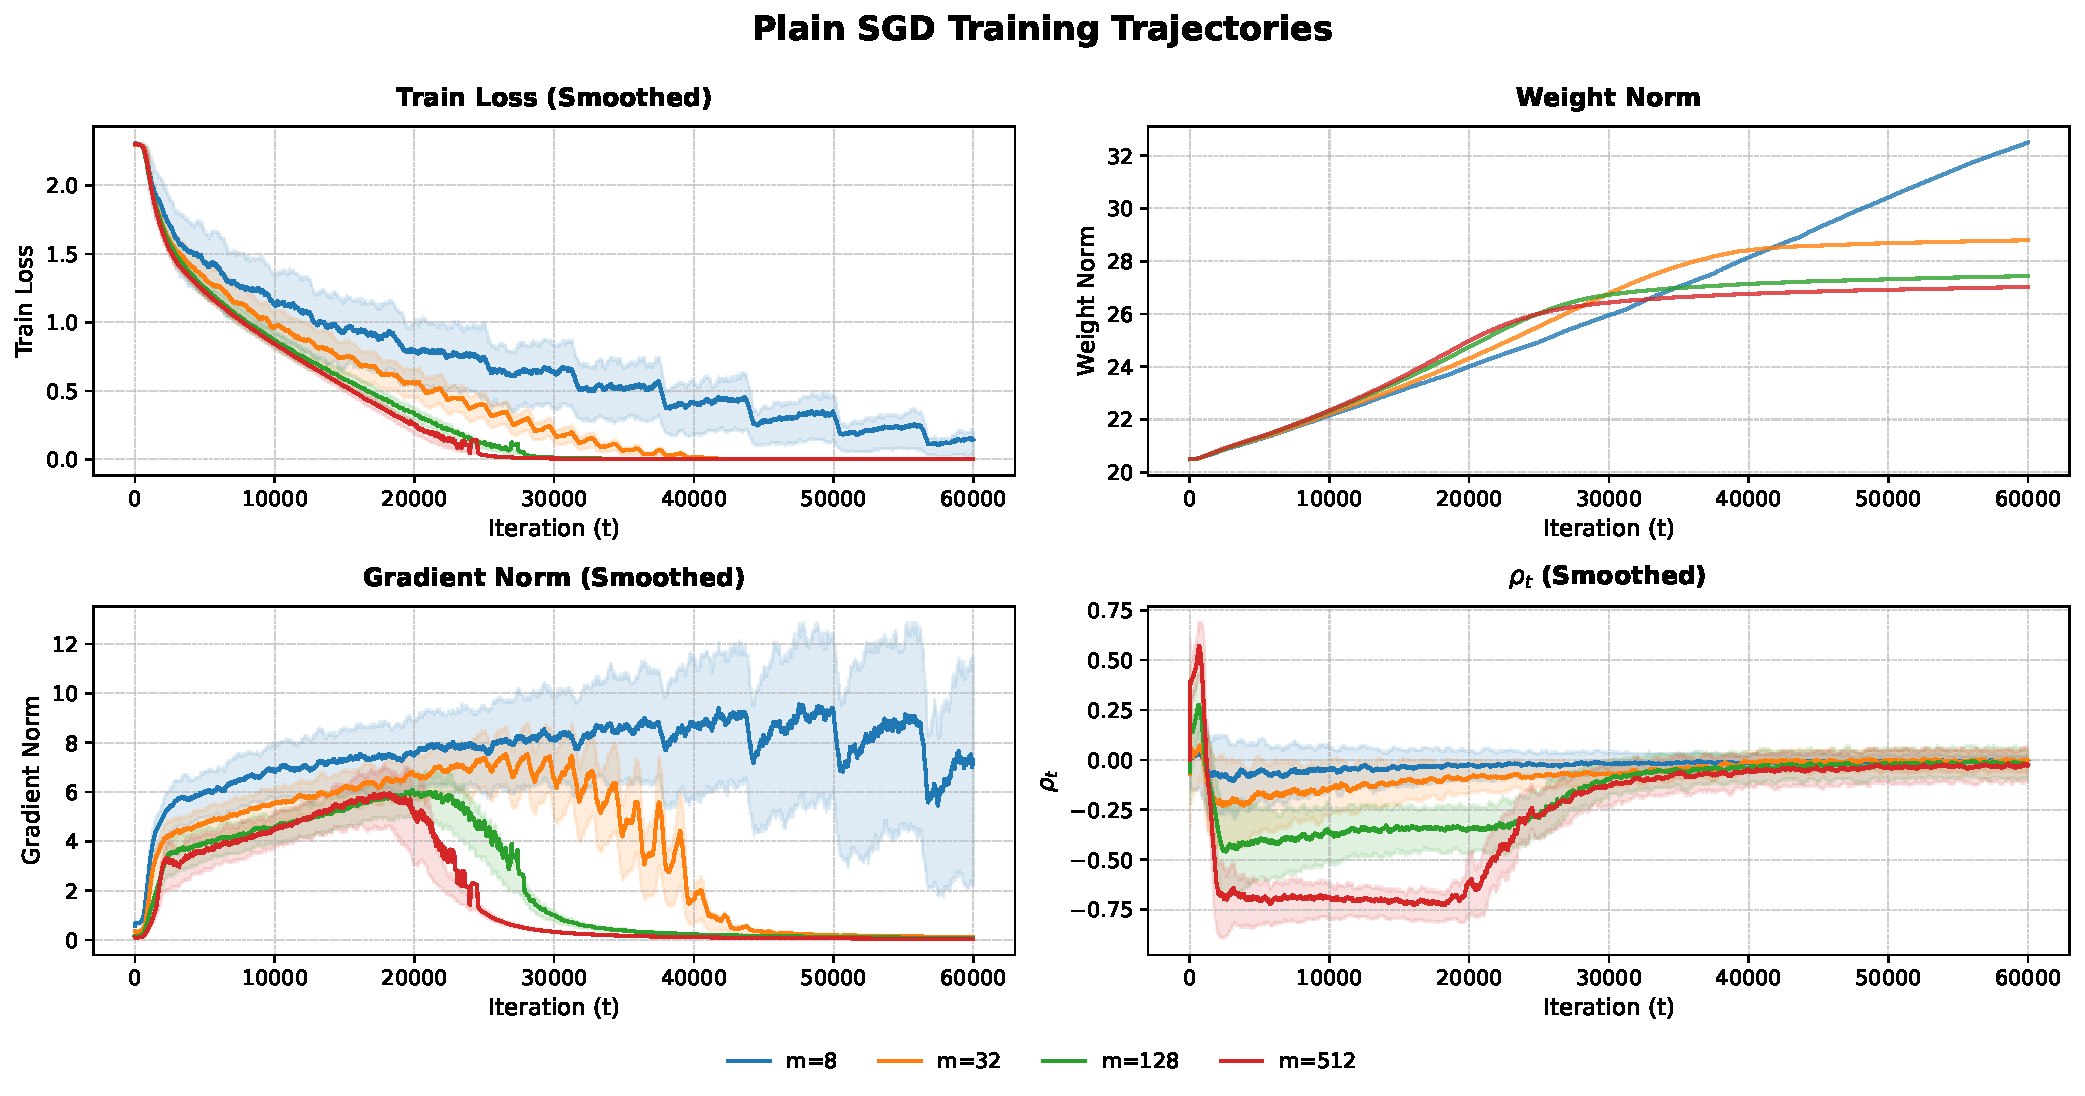
\includegraphics[width=1\linewidth]{figures/traj_metrics_cifar10_less_batches.pdf}
    \caption{Smoothed training trajectories for plain SGD with $\eta = 0.01$. The plot grid shows training loss, the model's weight norm, gradient norms, and the cosine similarity between the gradients of sequential batches.}
    \label{fig:cifar_traj}
\end{figure*}


Across all batch sizes, the training trajectories follow a consistent three-phase pattern. In the initial phase, successive gradients are strongly aligned, as indicated by positive cosine similarity, as shown in the bottom-right corner plot of Fig. \ref{fig:cifar_traj}. This alignment is stronger for larger batches and corresponds to rapid loss reduction and steady growth of the parameter norm, reflecting effective accumulation of the learning signal. As training progresses, an oscillatory phase emerges in which cosine similarity becomes negative. This indicates that successive updates partially oppose one another, consistent with overshooting and oscillation around a minimum. In the final phase, cosine similarity approaches zero, indicating that successive gradients are largely uncorrelated. In this regime, loss improvement saturates, and training becomes noise-dominated: parameter updates behave like a random walk, and further norm growth is driven primarily by stochastic fluctuations rather than a consistent learning signal.

Training dynamics vary systematically with batch size. For larger batches, the three phases are clearly separated, and the optimization trajectory is well structured. Gradient estimates are more accurate, leading to strong early alignment, a clear oscillatory phase near the minimum, and eventual convergence. As the batch size decreases, the magnitude of $\rho_t$ decreases, indicating weaker gradient alignment and larger stochasticity. For the smallest batch size (\(m = 8\)), training is largely noise-dominated: the loss and gradient norms fluctuate strongly, while the parameter norm continues to grow. In this regime, weight growth is driven primarily by stochastic noise rather than by a consistent learning signal, indicating that noise is being absorbed into the parameters without stable convergence.

%\subsection{Momentum}
\subsection{Momentum as Temporal Averaging}
\label{subsec:momentum_method}

Plain SGD exhibits an oscillatory regime in which consecutive updates partially cancel each other, leading to negative cross-step interference ($S_3<0$). Momentum mitigates this behavior by averaging gradients over time, thereby smoothing the trajectory and promoting more consistent update directions. Here, we consider SGD with momentum~\cite{polyak1964methods}. Let $\mu\in[0,1]$ be the momentum coefficient and $p_t\in\mathbb{R}^d$ the velocity, with $p_0=0$. The updates are

\begin{equation}
\label{eq:momentum_updates}
\begin{aligned}
  p_{t+1} &= \mu p_t + G_{B_t}(\theta_t),\\
  \theta_{t+1} &= \theta_t - \eta\, p_{t+1}.
\end{aligned}
\end{equation}
%with $G_{B_t}(\theta_t)=\frac{1}{m}\sum_{i=1}^m g_i^{(t)}$ and $g_i^{(t)}=\nabla_\theta\ell(\theta_t;x_i,y_i)$. 
Unrolling the recursion yields $p_{t+1}=\sum_{u=0}^{t}\mu^{t-u}G_{B_u}(\theta_u)$, and telescoping $\theta_{t+1}-\theta_t=-\eta p_{t+1}$ gives
\begin{equation}
\begin{aligned}
\label{eq:thetaT_momentum}
\theta_T
&=\theta_0-\eta\sum_{t=0}^{T-1}\alpha_t\,G_{B_t}(\theta_t),
\\
\alpha_t
&:=\sum_{r=0}^{T-1-t}\mu^r
=
\frac{1-\mu^{T-t}}{1-\mu}.
\end{aligned}
\end{equation}
%
Expanding the squared norm as in Eq.~\eqref{eq:s_def}, we obtain the momentum-weighted trade-off decomposition
\begin{equation}
\label{eq:thetaT_full_momentum}
\|\theta_T\|^{2}
=\|\theta_0\|^{2}
+ C^{(\mu)}
+\frac{\eta^{2}}{m^{2}}\bigl(S_1^{(\mu)}+S_2^{(\mu)}+S_3^{(\mu)}\bigr),
\end{equation}
where
\begin{align}
C^{(\mu)}
&:=
-2\frac{\eta}{m}\sum_{t=0}^{T-1}\sum_{i=1}^{m}\alpha_t\,\theta_0^{\top}g_i^{(t)},
\label{eq:C_mu}\\
S_1^{(\mu)}
&:=
\sum_{t=0}^{T-1}\alpha_t^2\sum_{i=1}^{m}\|g_i^{(t)}\|^2,
\label{eq:S1_mu}\\
S_2^{(\mu)}
&:=
\sum_{t=0}^{T-1}\alpha_t^2\sum_{i=1}^{m}\sum_{\substack{j=1\\ j\neq i}}^{m} g_i^{(t)\top}g_j^{(t)},
\label{eq:S2_mu}\\
S_3^{(\mu)}
&:=
2\sum_{t=0}^{T-1}\sum_{u=0}^{t-1}\alpha_t\alpha_u\sum_{i=1}^{m}\sum_{j=1}^{m} g_i^{(t)\top}g_j^{(u)}.
\label{eq:S3_mu}
\end{align}
%
From Eqs.~\eqref{eq:thetaT_momentum}--\eqref{eq:S3_mu}, momentum can be interpreted as a temporal averaging mechanism. Because each update direction \(p_{t+1}\) is an exponentially weighted average of recent mini-batch gradients, momentum smooths high-frequency batch-to-batch variation and tends to make successive updates more coherent. In the signal--interference decomposition, this typically reduces destructive cross-step cancellation and can shift the trajectory toward more constructive accumulation (\(S_3 > 0\)). At the same time, the coefficients \(\alpha_t\) show that earlier gradients have a larger cumulative influence on \(\theta_T\), since they continue to affect many future updates through the momentum recursion. This longer memory is beneficial when the descent direction changes slowly over time, but it can be harmful for abrupt direction changes. Such a mismatch can arise from heterogeneous mini-batches, rapid changes in local geometry, or simply an overly large learning rate, which causes the accumulated velocity to overshoot. In that regime, momentum no longer stabilizes the trajectory; instead, it can amplify stale directions and increase oscillatory behavior.

%\subsection{Weight Decay}
\subsection{Weight Decay as Recency Bias}
\label{subsec:weight_decay_method}

We next consider SGD with weight decay~\cite{krogh1991simple,loshchilov2017decoupled}. Let $\lambda\ge 0$ be the weight--decay coefficient. The update is% and assume $\eta\lambda<1$. The update is
\begin{equation}
\label{eq:weight_decay_updates}
\begin{aligned}
\theta_{t+1}
&= \theta_t-\eta\bigl(G_{B_t}(\theta_t)+\lambda\theta_t\bigr)\\
&= (1-\eta\lambda)\,\theta_t-\eta\,G_{B_t}(\theta_t).
\end{aligned}
\end{equation}
%with $G_{B_t}(\theta_t)=\frac{1}{m}\sum_{i=1}^m g_i^{(t)}$ and $g_i^{(t)}=\nabla_\theta\ell(\theta_t;x_i,y_i)$.
Unrolling the recursion yields, in the sample-level form, % the closed form
% \begin{equation}
% \label{eq:thetaT_weight_decay}
% \begin{aligned}
% \theta_T
% &= (1-\eta\lambda)^T\theta_0
% -\eta\sum_{t=0}^{T-1}(1-\eta\lambda)^{T-1-t}\,G_{B_t}(\theta_t).
% \end{aligned}
% \end{equation}
% In sample--level form,
\begin{equation}
\begin{aligned}
\theta_T
&= (1-\eta\lambda)^T\theta_0
-\frac{\eta}{m}\sum_{t=0}^{T-1}\sum_{i=1}^m (1-\eta\lambda)^{T-1-t}\,g_i^{(t)}.
\label{eq:wd_theta_T}
\end{aligned}
\end{equation}
%
Expanding the squared norm as in Eq.~\eqref{eq:s_def}, we obtain the weight--decayed trade-off decomposition
\begin{equation}
\begin{aligned}  
\label{eq:thetaT_full_wd}
\|\theta_T\|^{2}
&=(1-\eta\lambda)^{2T}\|\theta_0\|^{2}
+ C^{(\mathrm{wd})} \\
&+\frac{\eta^{2}}{m^{2}}\bigl(S_1^{(\mathrm{wd})}+S_2^{(\mathrm{wd})}+S_3^{(\mathrm{wd})}\bigr),
\end{aligned}
\end{equation}
where
\begin{align}
C^{(\mathrm{wd})}
&:=
-2\frac{\eta}{m}\sum_{t=0}^{T-1}\sum_{i=1}^{m}(1-\eta\lambda)^{2T-1-t}\,\theta_0^{\top}g_i^{(t)},
\label{eq:C_wd}\\
S_1^{(\mathrm{wd})}
&:=
\sum_{t=0}^{T-1}(1-\eta\lambda)^{2(T-1-t)}\sum_{i=1}^{m}\|g_i^{(t)}\|^2,
\label{eq:S1_wd}\\
S_2^{(\mathrm{wd})}
&:=
\sum_{t=0}^{T-1}(1-\eta\lambda)^{2(T-1-t)}\sum_{i=1}^{m}\sum_{\substack{j=1\\ j\neq i}}^{m} g_i^{(t)\top}g_j^{(t)},
\label{eq:S2_wd}\\
S_3^{(\mathrm{wd})}
&:=
2\sum_{t=0}^{T-1}\sum_{u=0}^{t-1}(1-\eta\lambda)^{2T-2-t-u}\sum_{i=1}^{m}\sum_{j=1}^{m} g_i^{(t)\top}g_j^{(u)}.
\label{eq:S3_wd}
\end{align}
Weight decay introduces an exponential recency bias along the optimization trajectory. From Eq.~\eqref{eq:wd_theta_T}, the gradient at step \(t\) appears in \(\theta_T\) with coefficient \((1-\eta\lambda)^{T-1-t}\). Hence, a gradient from an earlier step is multiplied by the shrinkage factor \(1-\eta\lambda\) more times before training ends, and therefore contributes less to the final parameters. The same pattern carries over to the norm decomposition. In \(S_1^{(\mathrm{wd})}\) and \(S_2^{(\mathrm{wd})}\), the contribution from step \(t\) is weighted by \((1-\eta\lambda)^{2(T-1-t)}\) because the coefficient of that step is squared in \(\|\theta_T\|^2\). In the cross-step term \(S_3^{(\mathrm{wd})}\), the interaction between steps \(t\) and \(u\) is weighted by \((1-\eta\lambda)^{2T-2-t-u}\), since it combines one factor \((1-\eta\lambda)^{T-1-t}\) from step \(t\) and one factor \((1-\eta\lambda)^{T-1-u}\) from step \(u\). Therefore, both individual contributions and pairwise interactions are increasingly suppressed as they originate farther in the past, while recent updates remain comparatively prominent. When \(\eta\lambda \ll 1\), this exponential decay yields an effective memory of approximately \((\eta\lambda)^{-1}\) steps. As a result, outdated gradients have limited influence on the parameter norm, which typically leads to more stable norm growth when the descent direction varies over time.

%\subsection{Ablations: SGD, Momentum, and Weight Decay}
\subsection{Stability Across Learning Rates and Batch Sizes}
\label{subsec:stability_ablations}

\begin{figure*}[t]
    \centering
    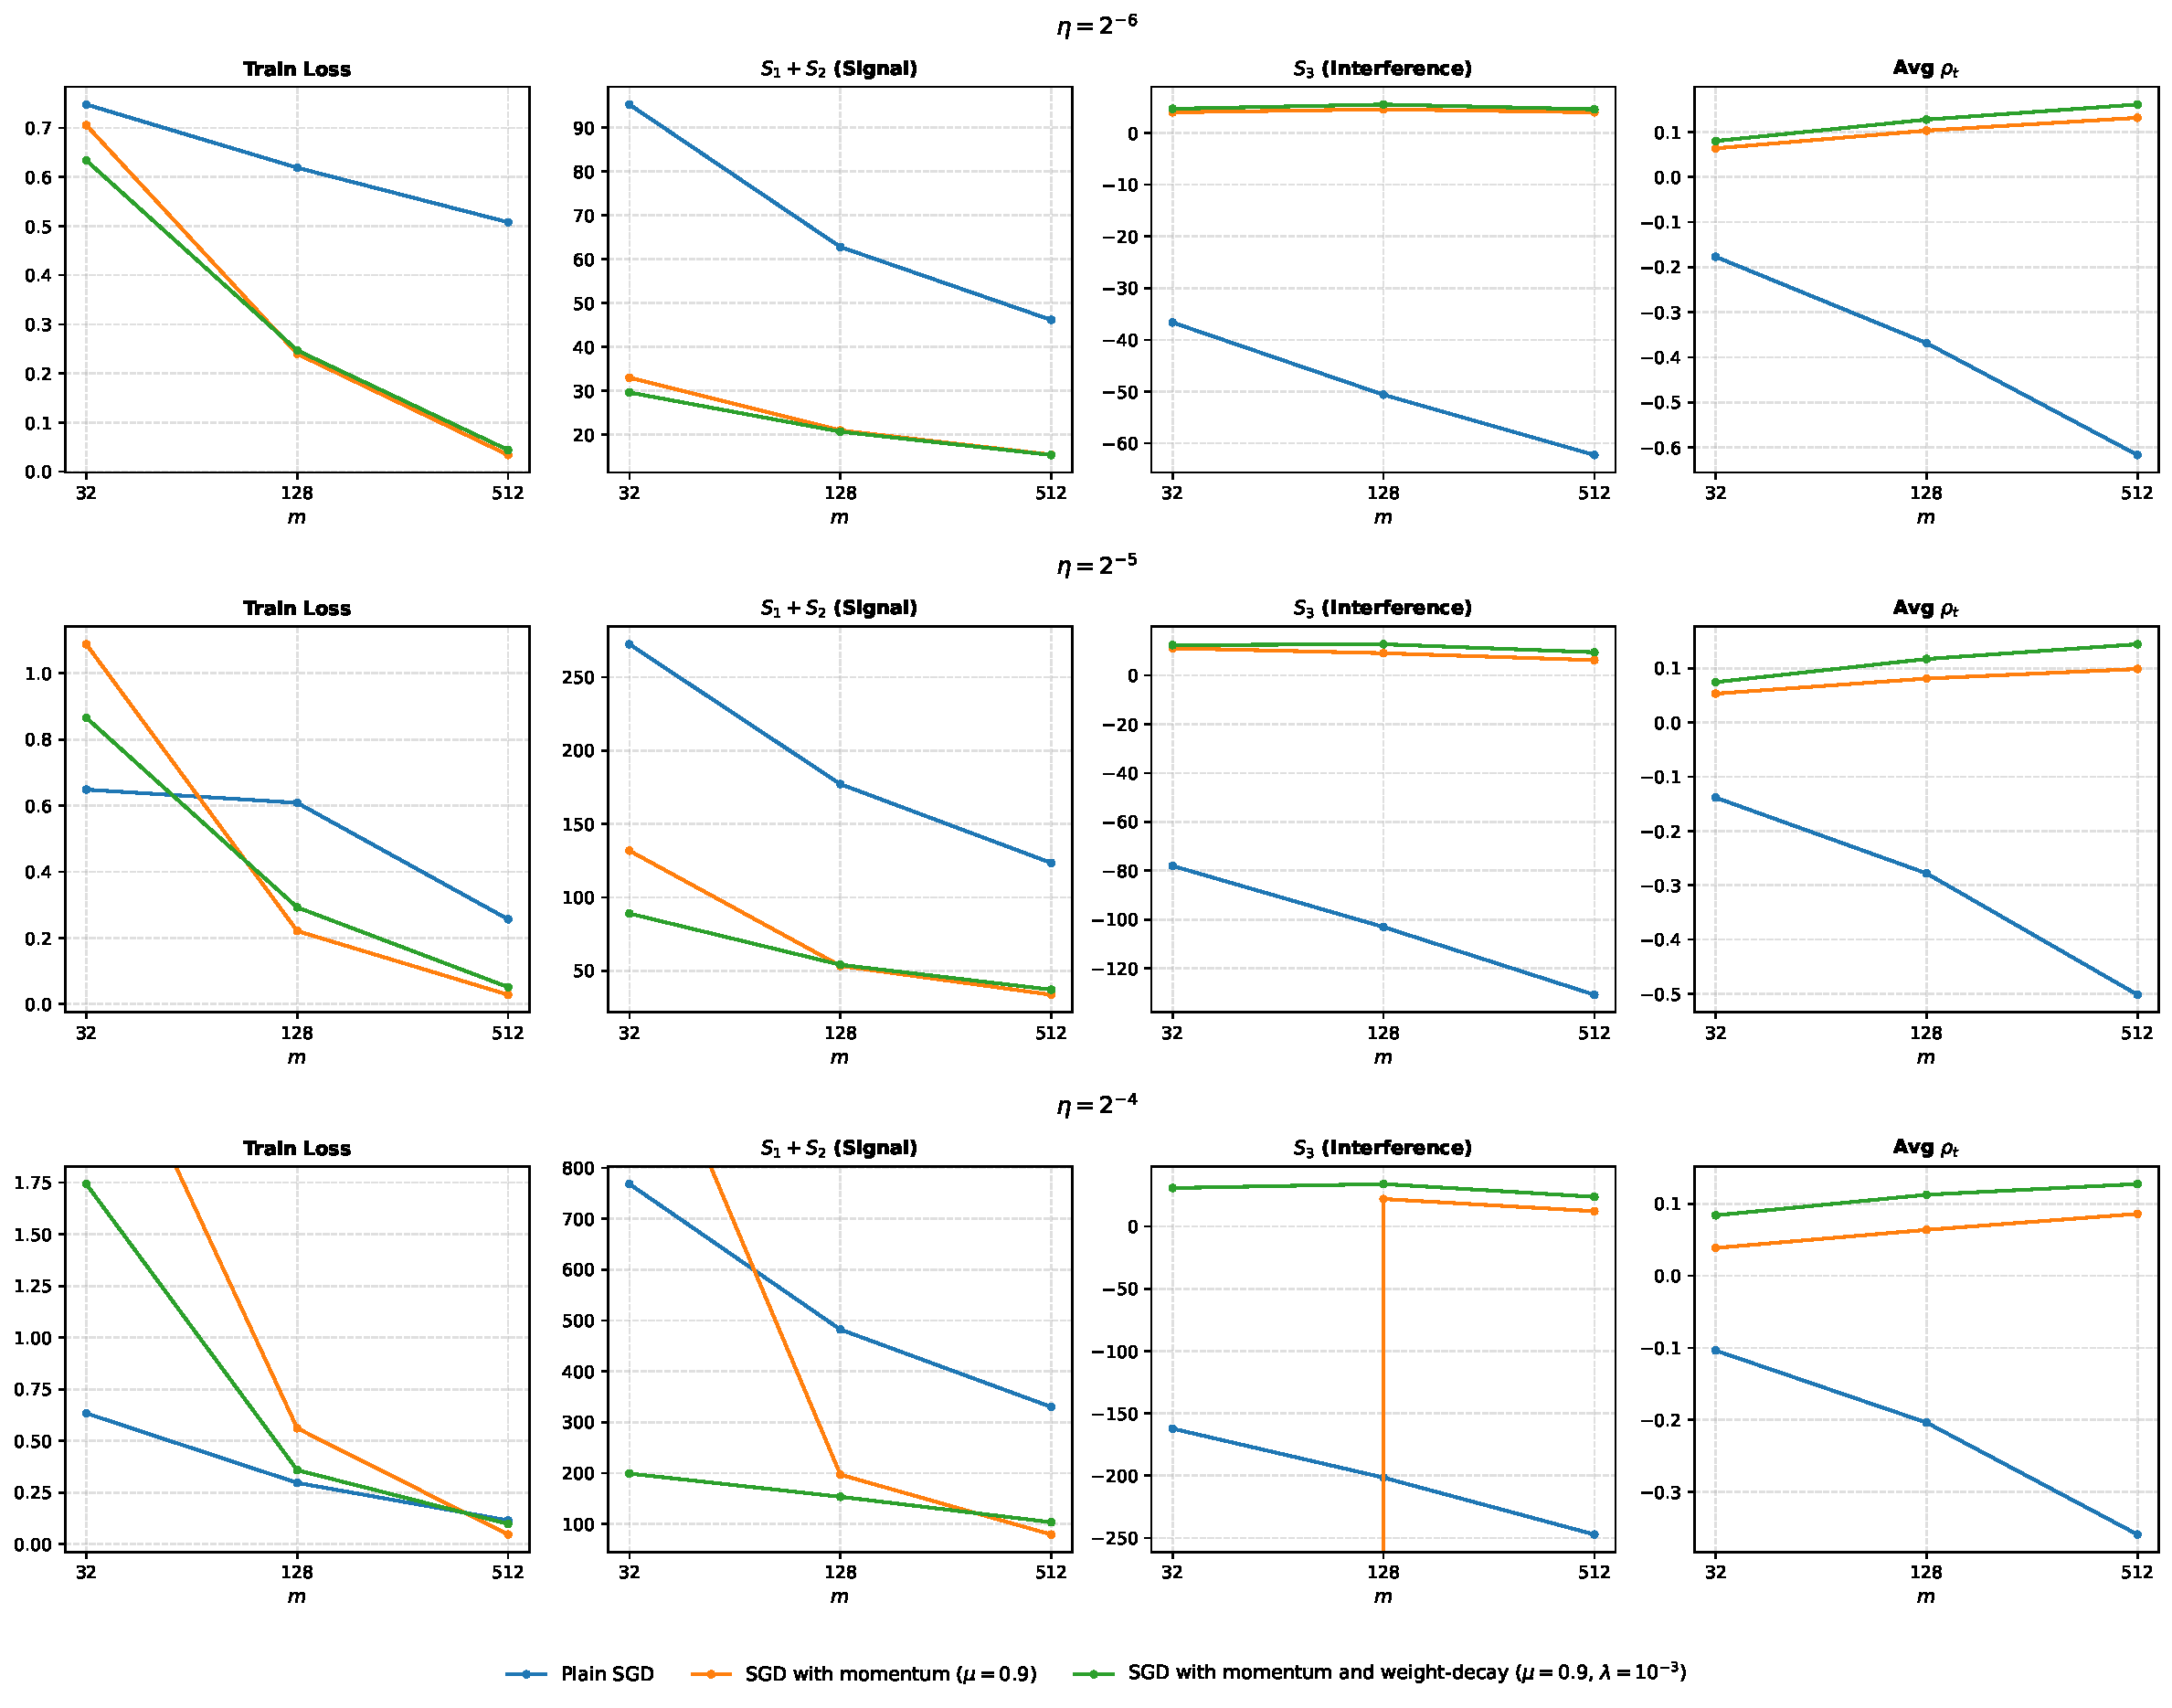
\includegraphics[width=0.95\linewidth]{figures/SGD_ablations_v2.pdf}
    \caption{\textbf{Empirical stability ablations for SGD, momentum, and weight decay.} We sweep batch size $m\in\{32, 128,512\}$ and learning rate $\eta\in\{2^{-6},2^{-5},2^{-4}\}$. Each point corresponds to a run and reports training loss, scaled signal $S_1+S_2$, scaled interference $S_3$, and the average consecutive-gradient cosine similarity $\overline{\rho}_t$.}
    \label{fig:stability_ablations}
\end{figure*}

We complement the preceding trajectory analysis with an aggregated view of stability across hyperparameters. We sweep the batch size over $m\in\{32,128,512\}$ and the learning rate over $\eta\in\{2^{-6},2^{-5},2^{-4}\}$ for plain SGD, SGD with momentum, and SGD with momentum and weight decay. Figure~\ref{fig:stability_ablations} reports the final training loss, the terminal scaled signal $\frac{\eta^2}{m^2}(S_1+S_2)$ and interference terms $\frac{\eta^2}{m^2}S_3$, and the average gradient cosine similarity $\overline{\rho}_t$. Unlike the trajectories discussed earlier, this sweep compares the behavior across methods at matched $(\eta,m)$. A central pattern is that larger batches improve all three methods, but they do so through different combinations of signal and interference.

Plain SGD remains in a destructive cross-step regime throughout the sweep. For every $\eta\in\{2^{-6},2^{-5},2^{-4}\}$ and every $m\in\{32,128,512\}$, the average gradient similarity is negative $(\overline{\rho}_t<0)$ and the corresponding cross-step term is also negative $(S_3<0)$. At a fixed learning rate, decreasing the batch size worsens the loss, increases $S_1+S_2$, and moves both $S_3$ and $\overline{\rho}_t$ toward zero. This shows that $S_1+S_2$ should not be interpreted directly as a more useful signal: it is an update-energy term, and it can grow simply because the gradients become noisier. The sweep suggests that reducing the batch size pushes plain SGD toward a noisy drift regime, whereas increasing it moves SGD toward a more coherent but more strongly interfering regime. Plain SGD thus appears to operate between two unfavorable extremes: random drift at small batch sizes and destructive interference at large batch sizes.

Introducing momentum $(\mu=0.9)$ moves the trajectory into a constructive regime ($\overline{\rho}_t>0$ and $S_3>0$) not seen in plain SGD. For $\eta\in\{2^{-6},2^{-5}\}$, the constructive cross-step coincides with lower loss, especially for $m\in \{128, 512\}$. At the more aggressive learning rate $\eta=2^{-4}$, however, we observe the failure mode of momentum: the loss increases sharply, $S_1+S_2$ grows dramatically, and $S_3$ exhibits an unbounded negative excursion. Increasing the batch size mitigates this effect by making consecutive gradients more coherent, which improves the quality of temporal averaging and restores the low-loss constructive regime. 

Adding weight decay further improves the momentum regime, mainly in the more aggressive settings. Its clearest benefit appears at $\eta=2^{-4}$, where it suppresses the growth of $S_1+S_2$ and avoids the extreme breakdown observed for momentum alone at $m=32$, preserving positive alignment. In this sense, weight decay makes the momentum regime less sensitive to aggressive hyperparameter choices, consistent with the recency-bias interpretation.

%\subsection{Batch Representativeness and Noise}
\subsection{Batch Representativeness and Trajectory Coherence}
\label{subsec:batch-representativeness}


\begin{figure*} [h]
    \centering
    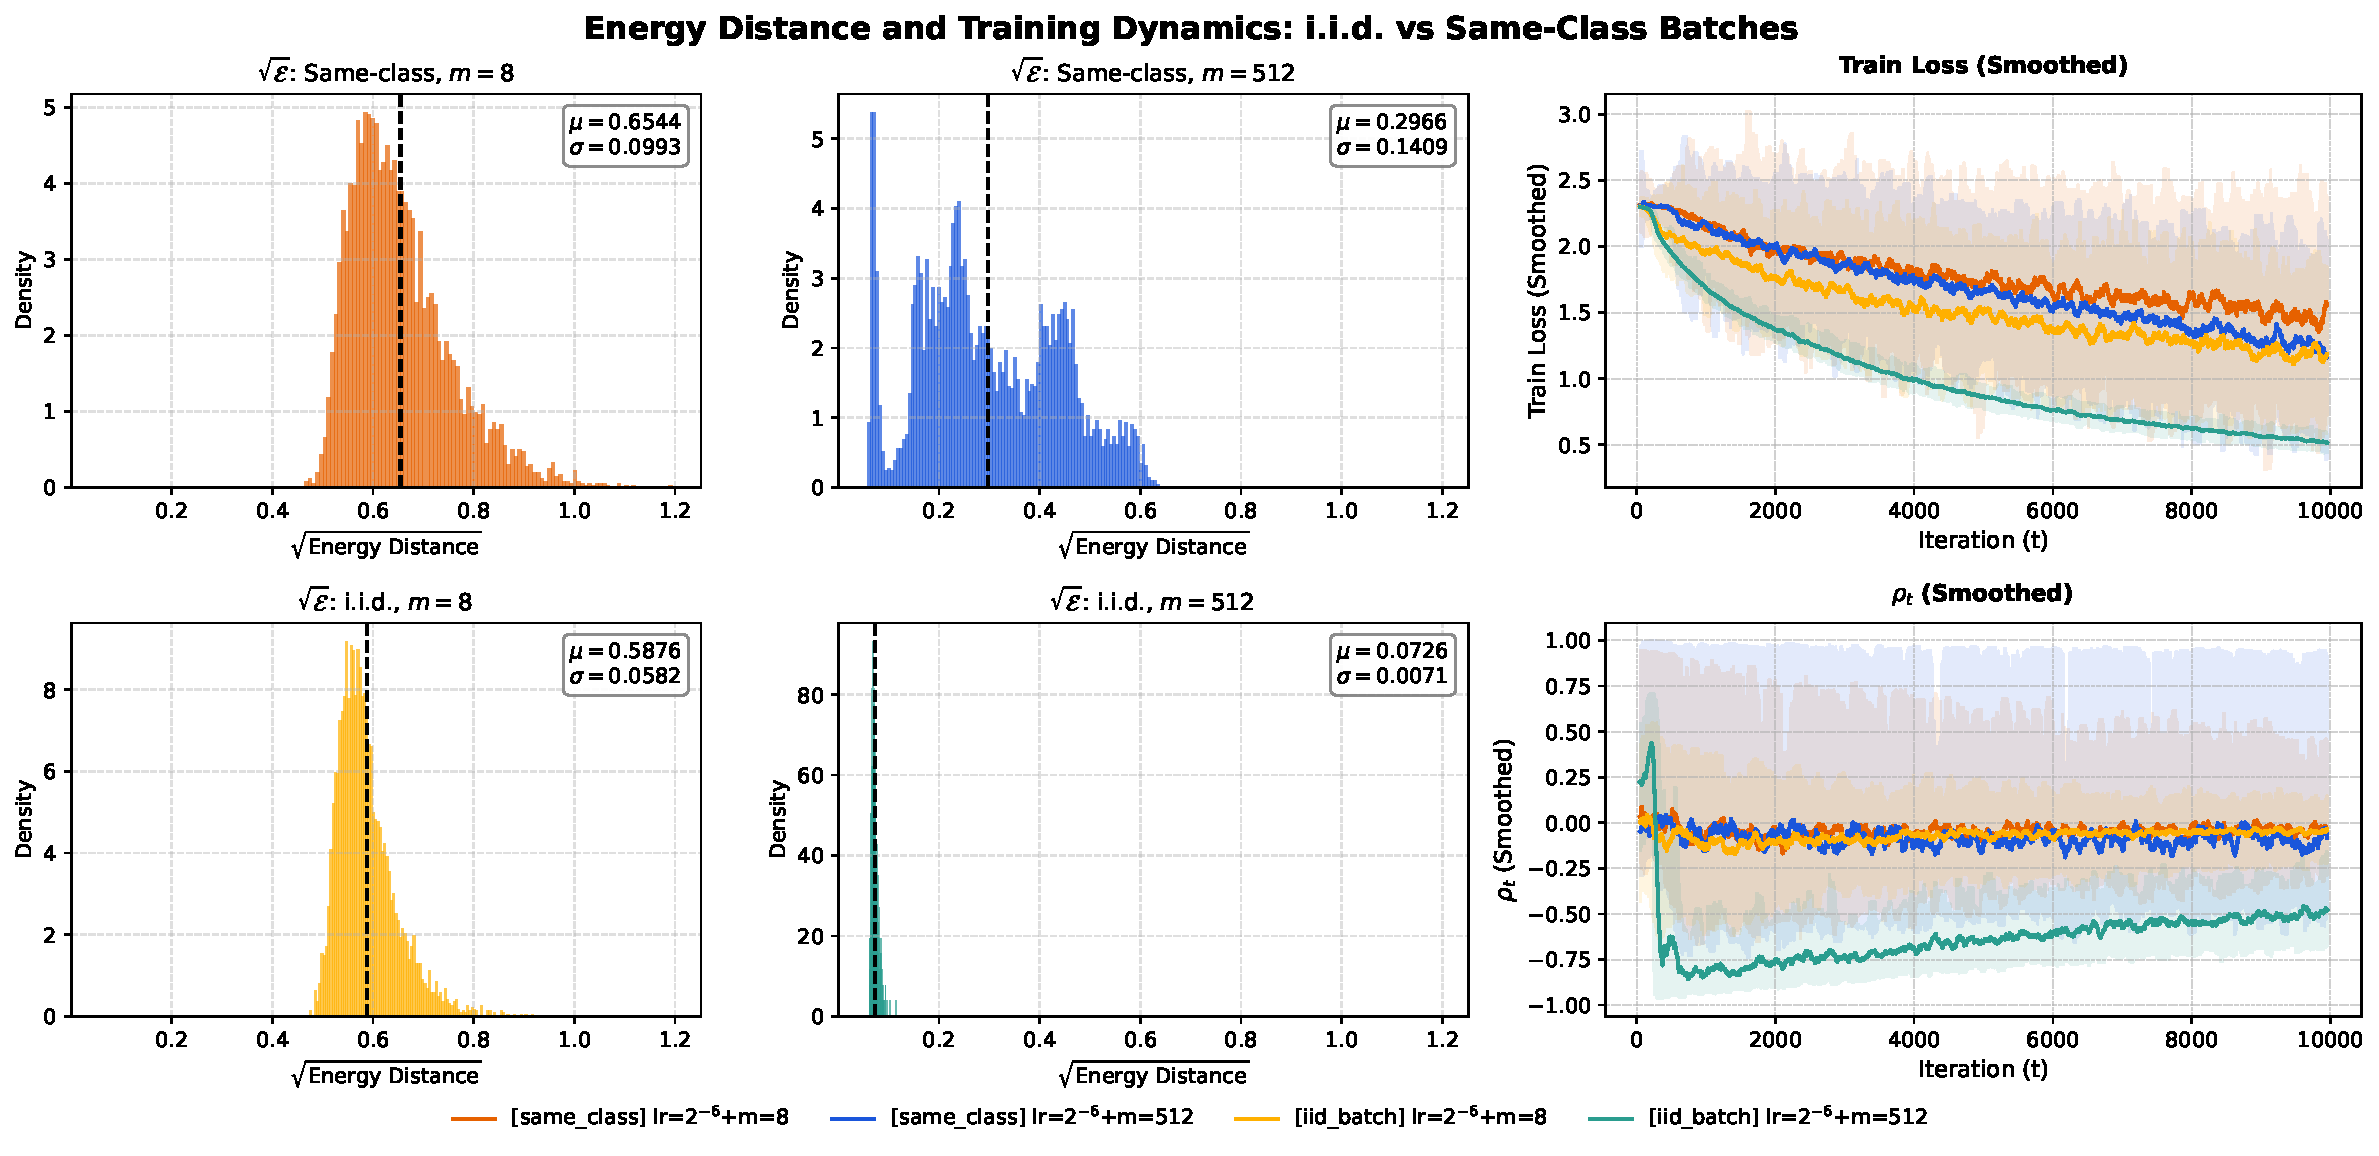
\includegraphics[width=1\linewidth]{figures/combined_energy_training_v2.pdf}
    \caption{\textbf{Effect of batch construction on consecutive-batch energy distance, and noisy trajectories at large batch sizes.} Histograms comparing same-class and i.i.d.\ sampling for $m=8$ and $m=512$. The horizontal axis shows $\sqrt{\mathcal{E}(X_{t-1},X_t)}$ (used to expand the scale for readability). Same-class sampling has a minor effect for $m=8$ ($\mu$: 0.58 $\to$ 0.65) but a large effect for $m=512$ ($\mu$: 0.07 $\to$ 0.29), indicating substantially higher inter-batch discrepancy at large batch sizes. Training loss and $\rho_t$ trajectories: same-class grouping prevents large batches from becoming representative, keeping consecutive updates weakly aligned (small average $\rho_t$) and yielding random-walk-like drift even at $m=512$.}
    \label{fig:energy_distance}
\end{figure*}



The ablations above suggest that training becomes less stable at small batch sizes because the trajectory becomes increasingly random, as indicated by \(\overline{\rho}_t \to 0\) for all cases. Here we argue that this effect is largely driven by limited batch representativeness. Under uniform sampling, each mini-batch \(X_t=\{\mathbf{x}_{t,i}\}_{i=1}^{m}\subset D\) provides only a finite approximation of the training distribution. When \(m\) is small, consecutive batches can differ substantially, leading to larger fluctuations in the gradient direction from one step to the next. As \(m\) increases, each batch becomes more representative of the dataset, and the resulting updates become more consistent across iterations.

Because our experiments use image data, we quantify batch representativeness directly in input space\footnote{For text data, an analogous notion of batch representativeness may be more naturally measured in embedding space, where distances can better reflect semantic similarity than raw token-space comparisons.} by measuring the \emph{energy distance} between consecutive mini-batches~\cite{szekely2013energy}. Given two successive batches, \(X_{t-1}=\{\mathbf{x}_i\}_{i=1}^{m}\) and \(X_t=\{\mathbf{x}_j\}_{j=1}^{m}\), we estimate this distance as
\begin{equation}
\begin{aligned}
\widehat{\mathcal{E}}(X_{t-1},X_t)
&=
\frac{2}{m^2}\sum_{i,j}\|\mathbf{x}_i-\mathbf{x}_j\| \\
&
-
\frac{1}{m(m-1)}\sum_{i\neq i'}\|\mathbf{x}_i-\mathbf{x}_{i'}\| \\
&
-
\frac{1}{m(m-1)}\sum_{j\neq j'}\|\mathbf{x}_j-\mathbf{x}_{j'}\|.
\end{aligned}
\label{eq:energy-sample}
\end{equation}
To effectively control \(\widehat{\mathcal{E}}(X_{t-1},X_t)\), we hold \(m\) fixed and break representativeness on purpose, violating the i.i.d.\ sampling assumption and constructing same-class mini-batches. Our hypothesis is as follows: assuming that batch size improves representativeness (i.e., reduces step-to-step energy distance), then breaking representativeness at a large batch size will reproduce small-batch interference dynamics and worse optimization behavior.
%If batch size helps primarily by improving representativeness (i.e., reducing step-to-step distance energy), then breaking it at a large batch size should reproduce small-batch interference dynamics and worse optimization behavior. 

Figure~\ref{fig:energy_distance} shows that the energy distance distribution between consecutive batches decreases with batch size under i.i.d.\ sampling, while breaking representativeness through same-class batching increases both its mean and variability. This effect is much stronger at \(m=512\) than at \(m=8\), suggesting that very small batches already operate far from the i.i.d.\ regime. The corresponding learning trajectories support this interpretation: when representativeness is disrupted, even large batches recover the noisy, weakly aligned dynamics usually associated with small-batch training. In particular, at fixed \(m=512\), cross-step interference collapses into random drift, and the updates accumulate more like a random walk than a consistent descent direction. These results suggest that much of the batch-size effect is mediated by representativeness: larger batches help because they make successive updates more statistically similar and therefore more temporally coherent. A natural conjecture is that this issue becomes more severe in the scaling regime: as input spaces grow and training data become more diverse, the representativeness of any fixed-size mini-batch should deteriorate, making cross-step coherence harder to maintain and training correspondingly more unstable.





\section{Conclusion}

The central claim of this paper is that the stability of SGD is not fully explained by pointwise properties of the loss landscape, such as local curvature. Instead, it also depends on temporal interactions between successive mini-batch updates, an aspect that remains comparatively underexplored despite its influence on the training trajectory. To address this gap, we introduced a signal--interference framework for stochastic optimization. By decomposing parameter growth into gradient signal and cross-step interference, the framework brings to light an important property of training dynamics: whether successive updates accumulate constructively or partially overwrite one another. We further derived a formulation to explain such interaction through consecutive-gradient cosine similarity, and used it to analyze plain SGD, momentum, and weight decay. Our results indicate that both stability and performance of SGD depend heavily on the combination of update magnitude and coherence. Momentum improves performance by making successive updates constructive, but it can become unstable if its velocity overshoots. Weight decay improves robustness by reducing the influence of older, stale directions. Overall, our findings complement existing approaches by introducing a temporal perspective on optimization dynamics, together with a practical diagnostic tool for assessing stability based on the correlation between successive updates. Therefore, these contributions provide a more mechanistic understanding of training evolution, helping to bridge the gap between theory and practice in modern machine learning.
% 
%%%%%%%%%%%%%%%%%%%%%%%%




% if have a single appendix:
%\appendix[Proof of the Zonklar Equations]
% or
%\appendix  % for no appendix heading
% do not use \section anymore after \appendix, only \section*
% is possibly needed

% use appendices with more than one appendix
% then use \section to start each appendix
% you must declare a \section before using any
% \subsection or using \label (\appendices by itself
% starts a section numbered zero.)
%


% \appendices
%\section{Proof of the First Zonklar Equation}
%Appendix one text goes here.

% you can choose not to have a title for an appendix
% if you want by leaving the argument blank
%\section{}
%Appendix two text goes here.

%\appendix[Two-Step Loss Reduction]
\appendices
\section{Sample-Level Decomposition for the Image-Classification Results}
\label{appendix:sample-level}

The image-classification results also report a sample-level decomposition.
For those results and this appendix, index mini-batches by $t=0,\ldots,T-1$,
write their size as $m$, and let $g_i^{(t)}$ be the gradient of sample $i$
evaluated at $\theta_t$. The batch mean is
\[
  G_{B_t}:=\frac{1}{m}\sum_{i=1}^m g_i^{(t)}.
\]
Thus, $G_{B_t}$ in this indexing is $g_{t+1}$ in
Section~\ref{sec:displacement}. For constant-step plain SGD,
\begin{equation}
  \theta_T=\theta_0-\eta\sum_{t=0}^{T-1}G_{B_t}.
  \label{eq:final_theta_expression}
\end{equation}
Taking the squared norm gives
\begin{equation}
\begin{aligned}
\|\theta_T\|^2={}&\|\theta_0\|^2
 -2\eta\sum_{t=0}^{T-1}\theta_0^\top G_{B_t}\\
 &+\eta^2\Bigl\|\sum_{t=0}^{T-1}G_{B_t}\Bigr\|^2.
\end{aligned}
\label{eq:norm_split_terms}
\end{equation}
Define the initialization--trajectory term
$C:=-2\eta\sum_{t=0}^{T-1}\theta_0^\top G_{B_t}$ and the sample-level sums
\begin{equation}
\begin{aligned}
S_1&:=\sum_{t=0}^{T-1}\sum_{i=1}^m\|g_i^{(t)}\|^2,\\
S_2&:=\sum_{t=0}^{T-1}\sum_{i=1}^m
       \sum_{\substack{j=1\\j\ne i}}^m g_i^{(t)\top}g_j^{(t)},\\
S_3&:=2\sum_{t=0}^{T-1}\sum_{u=0}^{t-1}
       \sum_{i,j=1}^m g_i^{(t)\top}g_j^{(u)}.
\end{aligned}
\label{eq:s_def}
\end{equation}
The sums collect per-sample energy, within-batch interactions, and all
cross-step interactions, respectively. Their expansion gives the exact identity
\begin{equation}
\begin{aligned}
\|\theta_T\|^2={}&\|\theta_0\|^2+C\\
 &+\frac{\eta^2}{m^2}(S_1+S_2+S_3).
\end{aligned}
\label{eq:thetaT_full}
\end{equation}
In particular, $(S_1+S_2)/m^2=\sum_t\|G_{B_t}\|^2$ is the batch-gradient
energy, while $S_3/m^2$ is the complete temporal interaction. The latter
cannot generally be recovered from consecutive cosine alone. These identities
specify the quantities displayed in Fig.~\ref{fig:traj_decomp}; they do not
identify their signs with loss reduction or a stability guarantee.

\begin{figure*}[h]
    \centering
    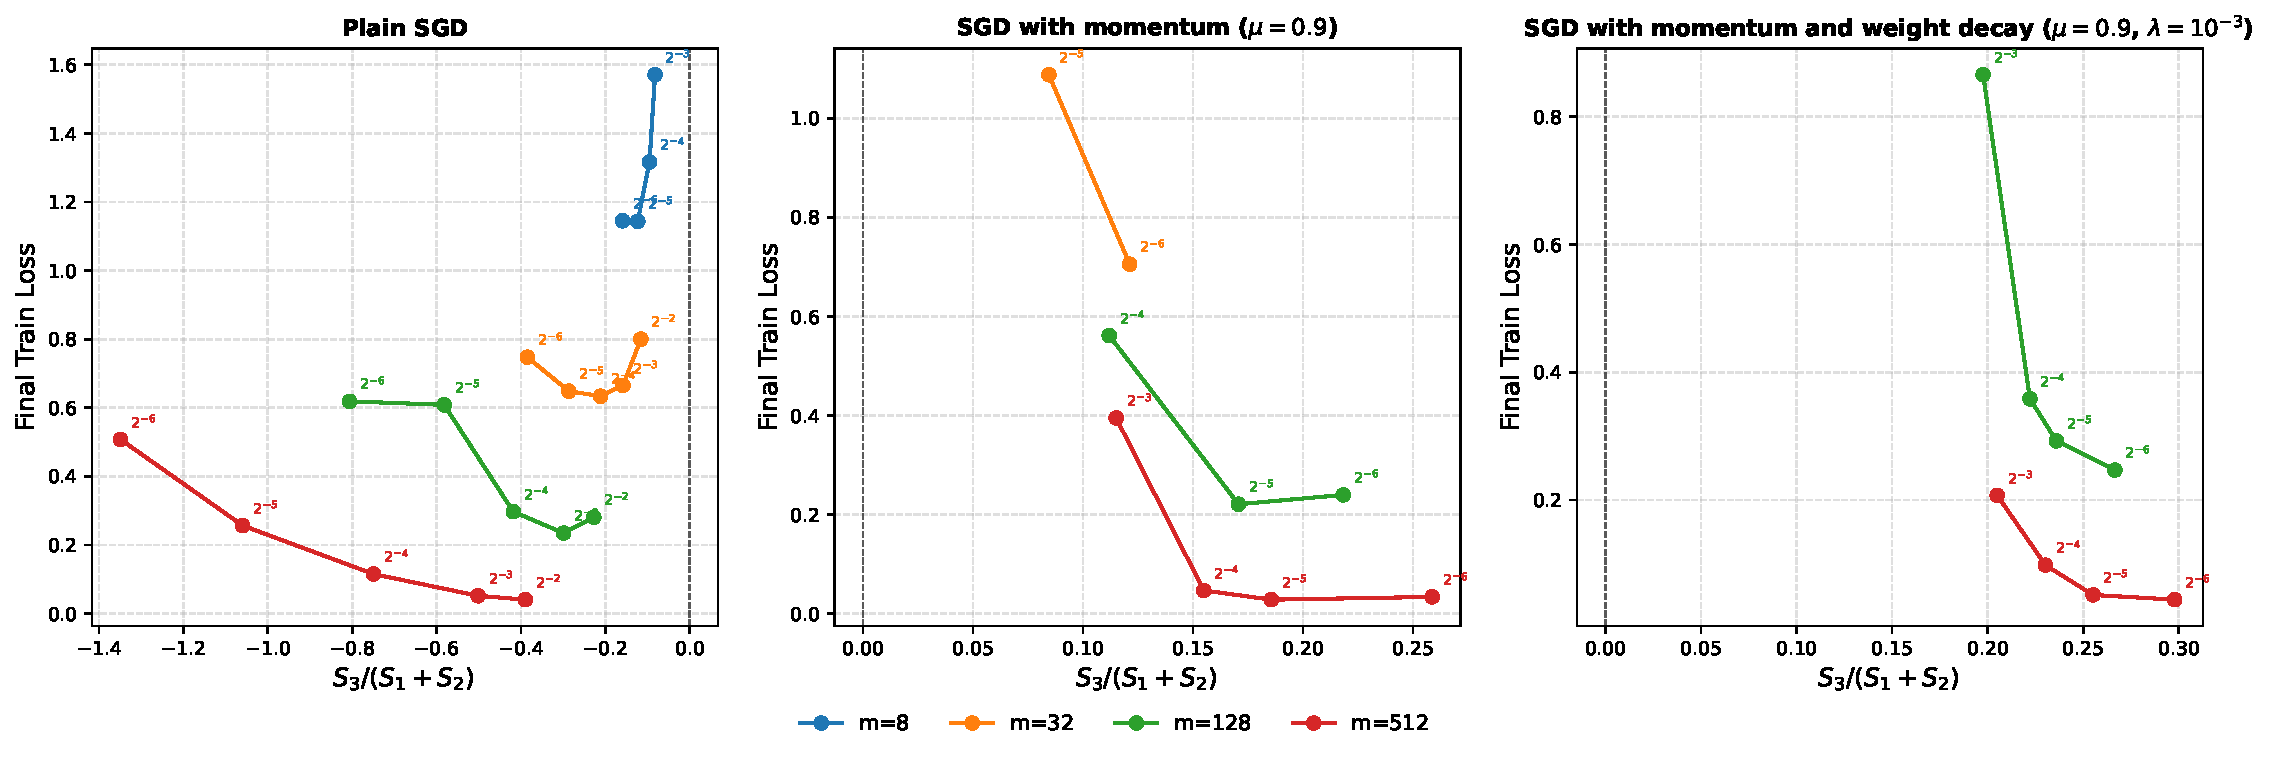
\includegraphics[width=1\linewidth]{figures/interf_ratio_to_loss.pdf}
    \caption{
Final training loss versus the normalized cross-step term \(S_3/(S_1+S_2)\) for VGG in CIFAR-10 with plain SGD (left), SGD with momentum \((\mu=0.9)\) (middle), and SGD with momentum plus weight decay \((\mu=0.9,\lambda=10^{-3})\) (right). Colors indicate batch size \(m\in\{8,32,128,512\}\); markers are annotated with the learning rate \(\{2^{-6}, ..., 2^{-2}\}\). The dashed vertical line denotes the boundary \(S_3=0\).
}
\label{fig:traj_decomp}
\end{figure*}

\section{Two-Step Loss Expansion}
\label{appendix:two_step}

This appendix uses the iteration indexing of Appendix~\ref{appendix:sample-level}: $G_{B_t}$ is evaluated at $\theta_t$, corresponding to $g_{t+1}$ in Section~\ref{sec:displacement}. Here the Hessian index likewise refers to $\theta_t$.

We derive Eq.~\eqref{eq:two_step_loss_interference} by combining a second-order Taylor expansion of the loss across two consecutive SGD steps with a first-order expansion of the gradient. Consider
\[
\theta_{t+1}=\theta_t-\eta\,G_{B_t},
\quad
\theta_{t+2}=\theta_{t+1}-\eta\,G_{B_{t+1}},
\]
and recall
\[
G_{B_t}=g^{(t)}+\xi_t,
\quad
g^{(t)}:=\nabla \mathcal{L}(\theta_t),
\quad
H_t:=\nabla^2\mathcal{L}(\theta_t).
\]
A second-order expansion of \(\mathcal{L}(\theta_{t+1})\) around \(\theta_t\) gives
\begin{equation}
\begin{aligned}
\mathcal{L}(\theta_{t+1})
&\approx
\mathcal{L}(\theta_t) \\
&-\eta\,g^{(t)\top}G_{B_t}
+\frac{\eta^2}{2}\,G_{B_t}^{\top}H_t\,G_{B_t}.
\end{aligned}
\label{eq:appendix_step1}
\end{equation}
Similarly, expanding \(\mathcal{L}(\theta_{t+2})\) around \(\theta_{t+1}\) yields
\begin{equation}
\begin{aligned}
\mathcal{L}(\theta_{t+2})
&\approx
\mathcal{L}(\theta_{t+1}) \\
&-\eta\,g^{(t+1)\top}G_{B_{t+1}}
+\frac{\eta^2}{2}\,G_{B_{t+1}}^{\top}H_{t+1}\,G_{B_{t+1}}.
\end{aligned}
\label{eq:appendix_step2}
\end{equation}
Next, using a first-order expansion of the gradient around \(\theta_t\),
\[
g^{(t+1)}
\approx
g^{(t)}+H_t(\theta_{t+1}-\theta_t)
=
g^{(t)}-\eta\,H_t\,G_{B_t},
\]
so that
\begin{equation}
-\eta\,g^{(t+1)\top}G_{B_{t+1}}
\approx
-\eta\,g^{(t)\top}G_{B_{t+1}}
+\eta^2\,G_{B_t}^{\top}H_t\,G_{B_{t+1}}.
\label{eq:appendix_grad_expand}
\end{equation}
Substituting Eqs.~\eqref{eq:appendix_step1} and \eqref{eq:appendix_grad_expand} into Eq.~\eqref{eq:appendix_step2}, we obtain
\begin{equation}
\label{eq:appendix_combined}
\begin{split}
\mathcal{L}(\theta_{t+2})
&\approx
\mathcal{L}(\theta_t)
-\eta\,g^{(t)\top}G_{B_t}
-\eta\,g^{(t)\top}G_{B_{t+1}} \\
&\quad
+\eta^2\,G_{B_t}^{\top}H_t\,G_{B_{t+1}}
+\frac{\eta^2}{2}\,G_{B_t}^{\top}H_t\,G_{B_t} \\
&\quad
+\frac{\eta^2}{2}\,G_{B_{t+1}}^{\top}H_{t+1}\,G_{B_{t+1}}.
\end{split}
\end{equation}
Using \(g^{(t)}=G_{B_t}-\xi_t\), the two first-order terms become
\[
g^{(t)\top}G_{B_t}
=
\|G_{B_t}\|^2-\xi_t^{\top}G_{B_t},
\]
\[
g^{(t)\top}G_{B_{t+1}}
=
G_{B_t}^{\top}G_{B_{t+1}}
-\xi_t^{\top}G_{B_{t+1}}.
\]
Thus,
\begin{equation}
\label{eq:appendix_pre_rho}
\begin{split}
\mathcal{L}(\theta_{t+2})
&\approx
\mathcal{L}(\theta_t)
-\eta\Bigl(
\|G_{B_t}\|^2
+
G_{B_t}^{\top}G_{B_{t+1}}
\Bigr) \\
&\quad
+\eta\,\xi_t^{\top}\!\bigl(G_{B_t}+G_{B_{t+1}}\bigr)
+\eta^2\,G_{B_t}^{\top}H_t\,G_{B_{t+1}} \\
&\quad
+\frac{\eta^2}{2}\Bigl(
G_{B_t}^{\top}H_t\,G_{B_t}
+
G_{B_{t+1}}^{\top}H_{t+1}\,G_{B_{t+1}}
\Bigr).
\end{split}
\end{equation}
Finally, by the definition of the cosine similarity between consecutive mini-batch gradients,
\[
\rho_{t+1}
=
\frac{G_{B_t}^{\top}G_{B_{t+1}}}
{\|G_{B_t}\|\,\|G_{B_{t+1}}\|},
\]
\[
G_{B_t}^{\top}G_{B_{t+1}}
=
\|G_{B_t}\|\,\|G_{B_{t+1}}\|\,\rho_{t+1}.
\]
Substituting this into Eq.~\eqref{eq:appendix_pre_rho} yields Eq.~\eqref{eq:two_step_loss_interference}.
\begin{equation}
\begin{aligned}
\mathcal{L}(\theta_{t+2})
&\;\approx\;
\mathcal{L}(\theta_t) \\
&\;-\;\eta\Big(\|G_{B_t}\|^2 \;+\; \|G_{B_t}\|\,\|G_{B_{t+1}}\|\,\rho_{t+1}\Big) \\
&\;+\;\eta\,\xi_t^{\top}\!\bigl(G_{B_t} + G_{B_{t+1}}\bigr) \\
&\;+\;\eta^2\, G_{B_t}^{\top} H_t\, G_{B_{t+1}} \\
&\;+\;\frac{\eta^2}{2}\Big(
G_{B_t}^{\top} H_t\, G_{B_t}
\;+\;
G_{B_{t+1}}^{\top} H_{t+1}\, G_{B_{t+1}}
\Big),
\end{aligned}
\label{eq:two_step_loss_interference}
\end{equation}




% use section* for acknowledgment
% \section*{Acknowledgment}

% The authors would like to thank...


% Can use something like this to put references on a page
% by themselves when using endfloat and the captionsoff option.
\ifCLASSOPTIONcaptionsoff
  \newpage
\fi



% trigger a \newpage just before the given reference
% number - used to balance the columns on the last page
% adjust value as needed - may need to be readjusted if
% the document is modified later
%\IEEEtriggeratref{8}
% The "triggered" command can be changed if desired:
%\IEEEtriggercmd{\enlargethispage{-5in}}

% references section

% can use a bibliography generated by BibTeX as a .bbl file
% BibTeX documentation can be easily obtained at:
% http://mirror.ctan.org/biblio/bibtex/contrib/doc/
% The IEEEtran BibTeX style support page is at:
% http://www.michaelshell.org/tex/ieeetran/bibtex/
\bibliographystyle{IEEEtran}
% argument is your BibTeX string definitions and bibliography database(s)
\bibliography{IEEEabrv,bibliography.bib}
%
% <OR> manually copy in the resultant .bbl file
% set second argument of \begin to the number of references
% (used to reserve space for the reference number labels box)
% \begin{thebibliography}{1}
% \end{thebibliography}

% biography section
% 
% If you have an EPS/PDF photo (graphicx package needed) extra braces are
% needed around the contents of the optional argument to biography to prevent
% the LaTeX parser from getting confused when it sees the complicated
% \includegraphics command within an optional argument. (You could create
% your own custom macro containing the \includegraphics command to make things
% simpler here.)
%\begin{IEEEbiography}[{\includegraphics[width=1in,height=1.25in,clip,keepaspectratio]{mshell}}]{Michael Shell}
% or if you just want to reserve a space for a photo:

% \begin{IEEEbiography}{Michael Shell}
% Biography text here.
% \end{IEEEbiography}

% \begin{IEEEbiographynophoto}{Thiago Mattar}
% received the B.Sc. degree in electrical engineering and the master's degree in electrical engineering from the Universidade Federal de Minas Gerais (UFMG), Brazil, in 2018 and 2022, respectively. He is currently pursuing a Ph.D. degree in Electrical Engineering at UFMG, with research focused on neural network learning techniques to enhance generalization and efficiency. Concurrently, he serves as Director and Quantitative Portfolio Manager at Alphabot, a proprietary hedge fund specializing in high-frequency trading and relative value arbitrage. His work bridges rigorous academic research and practical applications.
% \end{IEEEbiographynophoto}


% % if you will not have a photo at all:
% \begin{IEEEbiographynophoto}{Frederico Gualberto Ferreira Coelho}
% Biography text here.
% \end{IEEEbiographynophoto}


% \begin{IEEEbiographynophoto}{Cristiano Leite de Castro}
% Biography text here.
% \end{IEEEbiographynophoto}

% % insert where needed to balance the two columns on the last page with
% % biographies
% %\newpage

% \begin{IEEEbiographynophoto}{Antônio P. Braga}
% received the B.Sc. degree in electrical engineering and the master’s degree in computer science from the Universidade Federal de Minas Gerais (UFMG), Brazil, in 1987 and 1991, respectively, and the Ph.D. degree in electrical engineering from the University of London, Imperial College, in 1995, specializing in Recurrent Neural Networks. Since 1991, he has been with the Electronics Engineering Department at UFMG, where he is now a Full Professor and Head of the Computational Intelligence Laboratory. He is also an Associate Researcher at the Brazilian National Research Council. As a Professor and Researcher, he has co-authored numerous books, book chapters, journal, and conference papers. He serves as an Associate Editor for the Pattern Recognition and Engineering Applications of Artificial Intelligence.
% \end{IEEEbiographynophoto}

% You can push biographies down or up by placing
% a \vfill before or after them. The appropriate
% use of \vfill depends on what kind of text is
% on the last page and whether or not the columns
% are being equalized.

%\vfill

% Can be used to pull up biographies so that the bottom of the last one
% is flush with the other column.
%\enlargethispage{-5in}



% that's all folks
\end{document}


